\documentclass[12pt, a4paper]{article}

%%%%%%%%%%%%%%%%%%%%%%%%%%%%%%%%%%%%%%%%%
% Wenneker Article
% Structure Specification File
% Version 1.0 (28/2/17)
%
% This file originates from:
% http://www.LaTeXTemplates.com
%
% Authors:
% Frits Wenneker
% Vel (vel@LaTeXTemplates.com)
%
% License:
% CC BY-NC-SA 3.0 (http://creativecommons.org/licenses/by-nc-sa/3.0/)
%
% Adapted for COMS30007 by Carl Henrik Ek
% And then adapted for his Thesis by Leo Poulson
%
%%%%%%%%%%%%%%%%%%%%%%%%%%%%%%%%%%%%%%%%%

%----------------------------------------------------------------------------------------
%	PACKAGES AND OTHER DOCUMENT CONFIGURATIONS
%----------------------------------------------------------------------------------------

\usepackage[english]{babel} % English language hyphenation

\usepackage{microtype} % Better typography

\usepackage{amsthm} % Math packages for equations
\usepackage{amsmath}
\usepackage{amssymb}
\usepackage{mathtools}
\usepackage{bm}
\usepackage{xfrac}
\usepackage{resizegather}
\usepackage[]{algorithmicx}

\usepackage{minted}

\usepackage[weather]{ifsym}

\usepackage{wrapfig}


\usepackage[svgnames]{xcolor} % Enabling colors by their 'svgnames'

\usepackage[hang, small, labelfont=bf, up, textfont=it]{caption} % Custom captions under/above tables and figures

\usepackage{booktabs} % Horizontal rules in tables

\usepackage{lastpage} % Used to determine the number of pages in the document (for "Page X of Total")

\usepackage{graphicx} % Required for adding images

\usepackage{subcaption} % Add subfigures
\usepackage{enumitem} % Required for customising lists
\setlist{noitemsep} % Remove spacing between bullet/numbered list elements

\usepackage{sectsty} % Enables custom section titles
\allsectionsfont{\usefont{OT1}{phv}{b}{n}} % Change the font of all section commands (Helvetica)

\usepackage{tikz}

\usetikzlibrary{shapes.multipart} % Enables multi-line tikz nodes 
\usetikzlibrary{shapes.misc} % lets us use funny shapes
\usetikzlibrary{arrows,shapes,snakes,automata,backgrounds,petri}
\usetikzlibrary{positioning}

\usetikzlibrary{decorations.pathreplacing}

\usepackage{pgfplots}
\pgfplotsset{compat=1.9}
\usepgfplotslibrary{external}
%----------------------------------------------------------------------------------------
%	MARGINS AND SPACING
%----------------------------------------------------------------------------------------

\usepackage{geometry} % Required for adjusting page dimensions

\geometry{
	top=2cm, % Top margin
	bottom=2cm, % Bottom margin
	left=2cm, % Left margin
	right=2cm, % Right margin
	includehead, % Include space for a header
	includefoot, % Include space for a footer
	%showframe, % Uncomment to show how the type block is set on the page
}

\setlength{\columnsep}{7mm} % Column separation width

% --------------------------------------------------------
%   NEW COMMANDS
% --------------------------------------------------------

\newcommand{\mc}[1]{\mathcal{#1}}
\newcommand{\tmc}[1]{$\mathcal{#1}$}
\newcommand{\wh}[1]{\widehat{#1}}
\newcommand{\m}{\tmc{M}}
\newcommand{\e}{\tmc{E}}
\newcommand{\mm}{\mc{M}}
\newcommand{\me}{\mc{E}}
\newcommand{\rsarrow}{\rightsquigarrow}

\newcommand{\pre}{\textsf{pre}}
\newcommand{\post}{\textsf{post}}
\newcommand{\tpre}{$\pre$ }
\newcommand{\tpost}{$\post$ }

\newcommand{\mestar}{$\mathcal{ME^\ast}$ }

\newcommand{\secref}[1]{Section \ref{#1}}
\newcommand{\figref}[1]{Figure \ref{#1}}

\newcommand{\mih}[1]{\mintinline{haskell}{#1}}

% --------------------------------------------------------
%   NEW ENVIRONMENTS
% --------------------------------------------------------

\newenvironment{centermath}
 {\begin{center}$\displaystyle}
 {$\end{center}}

%----------------------------------------------------------------------------------------
%	FONTS
%----------------------------------------------------------------------------------------

\usepackage[T1]{fontenc} % Output font encoding for international characters
\usepackage[utf8]{inputenc} % Required for inputting international characters

\usepackage{XCharter} % Use the XCharter font

%----------------------------------------------------------------------------------------
%	HEADERS AND FOOTERS
%----------------------------------------------------------------------------------------

\usepackage{fancyhdr} % Needed to define custom headers/footers
\pagestyle{fancy} % Enables the custom headers/footers

\renewcommand{\headrulewidth}{0.0pt} % No header rule
\renewcommand{\footrulewidth}{0.4pt} % Thin footer rule

\renewcommand{\sectionmark}[1]{\markboth{#1}{}} % Removes the section number from the header when \leftmark is used

%\nouppercase\leftmark % Add this to one of the lines below if you want a section title in the header/footer

% Headers
\lhead{} % Left header
\chead{\textit{\thetitle}} % Center header - currently printing the article title
\rhead{} % Right header

% Footers
\lfoot{} % Left footer
\cfoot{} % Center footer
\rfoot{\footnotesize Page \thepage\ of \pageref{LastPage}} % Right footer, "Page 1 of 2"

\fancypagestyle{firstpage}{ % Page style for the first page with the title
	\fancyhf{}
	\renewcommand{\footrulewidth}{0pt} % Suppress footer rule
}

%----------------------------------------------------------------------------------------
%	TITLE SECTION
%----------------------------------------------------------------------------------------

\newcommand{\authorstyle}[1]{{\large\usefont{OT1}{phv}{b}{n}\color{DarkRed}#1}} % Authors style (Helvetica)

\newcommand{\institution}[1]{{\footnotesize\usefont{OT1}{phv}{m}{sl}\color{Black}#1}} % Institutions style (Helvetica)

\usepackage{titling} % Allows custom title configuration

\newcommand{\HorRule}{\color{DarkGoldenrod}\rule{\linewidth}{1pt}} % Defines the gold horizontal rule around the title

\pretitle{
	\vspace{-30pt} % Move the entire title section up
	\HorRule\vspace{10pt} % Horizontal rule before the title
	\fontsize{32}{36}\usefont{OT1}{phv}{b}{n}\selectfont % Helvetica
	\color{DarkRed} % Text colour for the title and author(s)
}

\posttitle{\par\vskip 15pt} % Whitespace under the title

\preauthor{} % Anything that will appear before \author is printed

\postauthor{ % Anything that will appear after \author is printed
	\vspace{10pt} % Space before the rule
	\par\HorRule % Horizontal rule after the title
	\vspace{20pt} % Space after the title section
}

%----------------------------------------------------------------------------------------
%	ABSTRACT
%----------------------------------------------------------------------------------------

\usepackage{lettrine} % Package to accentuate the first letter of the text (lettrine)
\usepackage{fix-cm}	% Fixes the height of the lettrine

\newcommand{\initial}[1]{ % Defines the command and style for the lettrine
	\lettrine[lines=3,findent=4pt,nindent=0pt]{% Lettrine takes up 3 lines, the text to the right of it is indented 4pt and further indenting of lines 2+ is stopped
		\color{DarkGoldenrod}% Lettrine colour
		{#1}% The letter
	}{}%
}

\usepackage{xstring} % Required for string manipulation

\newcommand{\lettrineabstract}[1]{
	\StrLeft{#1}{1}[\firstletter] % Capture the first letter of the abstract for the lettrine
	\initial{\firstletter}\textbf{\StrGobbleLeft{#1}{1}} % Print the abstract with the first letter as a lettrine and the rest in bold
}

%----------------------------------------------------------------------------------------
%	BIBLIOGRAPHY
%----------------------------------------------------------------------------------------

\usepackage[backend=bibtex,style=authoryear]{biblatex} % Use the bibtex backend with the authoryear citation style (which resembles APA)

\addbibresource{biblio.bib} % The filename of the bibliography

\usepackage[autostyle=true]{csquotes} % Required to generate language-dependent quotes in the bibliography


\title{Protocol Synthesis in the Dynamic Gossip Problem} % The article title

\author{
	\authorstyle{Leo Poulson}
	\newline\newline % Space before institutions
}

\date{\today}

\begin{document}

\maketitle
\thispagestyle{firstpage}

\tableofcontents
\newpage

\section{Introduction}

Planning is the task of computing a set of actions to take some state within a
model to a successful state. In such a model we have a set of \textit{actors},
who will perform these actions that we search for.

Planning, as put forward in \cite{PlanningBook}, covers a wide range of
applications; from making a robot enter a room to synchronising multiple
computers working on the same document. In this project we concern ourselves
with a special case of planning; namely \textit{epistemic planning}. In this we
begin with a state embodying the knowledge states for a set of agents. We then
want to compute a set of actions the agents may perform in order to take the
knowledge state of the agents to a successful one.

Epistemic planning is a relatively young area of research, first put forward in
\cite{BolanderEP}. It rests upon work done in Dynamic Epistemic Logic, which is
a logic used to reason about knowledge and how it is changed by actions. Despite
epistemic planning being proved to be undecidable in a lot of cases
\footnote{It is undecidable for models where the number of agents is greater
  than 1 (\cite{UndecidabilityEP}), and also in single-agent models where the
  accessibility relation is not an equivalence relation. It is however decidable
  for models where the event models are propositional (\cite{DecidabilityEp}).},
interest in the area has been maintained since its birth
(\cite{AutomataTechniques}), leading to the work that this project uses.

\bigskip

The gossip problem is a problem regarding peer-to-peer information sharing. A
set of agents start out with some \textit{secret information}, and their goal is
to transfer this information across the network, such that every other agent
finds out their secret. We call an agent who knows the secret of every other
agent to be an \textit{expert}; we want to reach a state where every agent is an
expert. When two agents communicate they tell each other all of the secrets they
know; hence the slightly frivolous but very apt title of the \textit{gossip}
problem.

The gossip problem was first put forward in \cite{Tijdeman:1971}, and was such
that each agent began with the phone number of every other agent. We can hence
visualise the set of agents as nodes and the fact of agent $a$ knowing the phone
number of $b$ as a directed edge, and so such a formulation would be a complete
graph as in \figref{fig:classicgossipex}.
colour

\bigskip

\begin{figure}[h]
  \centering
  \begin{subfigure}[c]{0.4\textwidth}
    \centering
    \begin{tikzpicture}
      [every node part/.style={align=center}]
      \node (a) [] at (0, 3) {$a$};
      \node (b) [] at (3, 3) {$b$};
      \node (c) [] at (0, 0) {$c$};
      \node (d) [] at (3, 0) {$d$};

      \draw [<->, dashed] (a) -- (b);
      \draw [<->, dashed] (a) -- (c);
      \draw [<->, dashed] (a) -- (d);
      \draw [<->, dashed] (b) -- (c);
      \draw [<->, dashed] (b) -- (d);
      \draw [<->, dashed] (c) -- (d);
    
    \end{tikzpicture}
    \caption{An example of a gossip graph in the classical formulation.}
    \label{fig:classicgossipex}
  \end{subfigure}%
  ~
  \begin{subfigure}[c] {0.4\textwidth}
    \centering
    \begin{tikzpicture}
      [every node part/.style={align=center}]
      \node (a) [] at (0, 3) {$a$};
      \node (b) [] at (3, 3) {$b$};
      \node (c) [] at (0, 0) {$c$};
      \node (d) [] at (3, 0) {$d$};
      
      \draw [->, dashed] (b) -- (d);
      \draw [<->, dashed] (a) -- (c);
      \draw [->, dashed] (b) -- (c);
    \end{tikzpicture}
    \caption{An example of an incomplete gossip graph. }
    \label{fig:dynamicgossipex}

  \end{subfigure}
  \caption{Some exemplar gossip graphs.}
\end{figure}

Recently a variation of this problem has been studied, entitled the
\textit{dynamic} gossip problem(\cite{DynamicGossip}, \cite{EpProforDyGo}). This
is a popular research topic, with applications in the study of epidemics and
information discovery (\cite{DiscoverythruGossip}, \textbf{Find some more
  refs}). In these scenarios our network may model some peer to peer network
where our agents are computers, where the goal is to find the IP addresses of
all of the other computers in the network; or a social network, where our nodes
are people who want to connect with every other user in their circle of friends. 

In this, we begin with each agent knowing some subset of the phone
numbers of every other agent. Hence a starting configuration of the dynamic
gossip problem may look like \figref{fig:dynamicgossipex}. When two agents
converse on the phone, they also exchange all of the phone numbers that they
know as well as all of the secrets. As such, the graph's edges increase in
number as phone calls occur.

\subsection{Existing Software}

As research work is done into a topic, it is only natural that software is
developed to support it. The three related pieces of software are
\cite{DEMO-S5}, \cite{SMCDEL} and \cite{GithubGossip}. These three tools are all
\textit{model checkers} for dynamic epistemic logic. A model checker is a
program that, given a model \tmc{M} and a formula $\phi$, tells the user whether
or not $\mc{M} \models \phi$. Given the setting, they specifically answer the
question ``given an initial state and a set of events, does the state reached by
the occurrence of these events at the initial state satisfy some property?''.

We can see model checking as the \textit{dual} of planning; in planning we want
to find such a sequence of events, whilst model checking verifies that these
events do indeed bring the system to a successful state. \cite{GithubGossip} is
also capable of planning, however in a na{\"i}ve way; it enumerates the set of
all possible calls and then checks if any of these are successful. As we see
later, this is a very inefficient method for planning. 

Despite this, there does not exist any software to solve the epistemic planning
problem as envisioned in the literature; indeed, the only software to solve any
epistemic planning problem is restricted to just gossip models.

\subsection{Contributions}

At a high level, our aim in this project is to put forward a process to solve
the planning problem for epistemic models and propositional event models. This
is motivated by the dynamic gossip problem; despite the literature on the topic
there is little work done on the topic of planning for it. Dynamic Gossip can be
modelled perfectly by epistemic models and propositional event models, and hence
is a very fitting case study for the tool we will develop. Although our
algorithm is designed to work for any models, it is hoped that the work done in
this thesis can shed light on how a specialised process could be designed for
the dynamic gossip problem.

Our process uses the algorithm outlined in \cite{AutomataTechniques}. This paper
provides an outline of an algorithm which could be used, however much work
remains to be done in order to make this outline into an implementable
algorithm. 

As a testament to the functionality of the algorithm, we give an implementation
of the process in Haskell. There is currently no existing algorithm or software
that performs planning for epistemic models. 

This process will entail use of automata, a method discussed in the literature
however yet to be formalised to the point at which it can be implemented, nor
implemented. The literature surrounding the task spans from epistemic logic to
game theory, and as such is far outside the reach of the standard degree
content. In this thesis we hope to present all of the related literature in a
simple manner, so that the reader may understand all of the concepts used. 

\bigskip

This project puts forward several challenges. The first challenge is compiling
the assorted literature on the topic. As we come to see later, the literature
stretches very far and wide; the collection, comprehension and recollection of
this literature is a substantial piece of work in itself.

\bigskip

The second is the act of designing the algorithm that we will use to solve the
planning problem. Whilst the algorithm is roughly laid out in
\cite{AutomataTechniques} and \cite{UniformStrategies}, this is but a sketch.
There still remains a lot of work to be done on it in order to make it an easy
to understand and implement process. The development of this forms our second
challenge.

\bigskip

The third is the implementation in Haskell of the designed process. Due to
Haskell's syntactic similarity to the mathematical notation we use to formalise
the problem\footnote{This similarity is discussed again later, and is one of the
  reasons Haskell was chosen for the task.} this is easier than it would be in
some languages, however this still has its difficulties.

\subsection{Aims}

Concretely, our aims are as follows:

\begin{itemize}
  \item Research and survey the literature on the topic of planning and the
    gossip problem, with an aim to combining them.
  \item Review the extant software on model checking and planning for epistemic
    models, with an aim to drawing comparions between the existing tools and the
    one developed. 
  \item Design an algorithm to solve the planning problem for epistemic models
    and propositional event models.
  \item Provide an implementation of the developed algorithm in Haskell.
  \item Design and implement a testing system, to check the correctness of the
    program and also aid with profiling.
  \item Perform a study of performance in terms of time and space, and explain
    any strengths or shortcomings in comparison to existing tools. 
\end{itemize}

% We hope that the work done in this thesis can help to unify work done on both
% dynamic gossip and epistemic planning, and

\subsection{Road Map}

In Section 2, we introduce, formalise and explain the concepts and tools needed
to understand the work in the rest of the thesis. This constitutes the first of
our challenges; collecting and displaying all of the surrounding literature in a
pleasant, simple manner is a goal of this thesis and this section achieves this.

In Section 3 we put forward the algorithm we designed in order to solve the
epistemic planning problem. This uses a simplified version of the process put
forward in \secref{sec:PowersetAutomata}. We also give an exemplar execution of
the algorithm, in order to show how it functions.

Section 4 discusses the Haskell implementation of the algorithm designed in
Section 3. We discuss the design decisions taken throughout the implementation,
including motivation for the use of Haskell to solve this problem.

In Section 5 we evaluate the algorithm and its implementation. To do this we
use \cite{GithubGossip} as both a model checker, to validate our results
returned from our planning tool, and also as a tool capable of planning, in
order to analyse the space and time efficiency of our tool. 

In Section 6 we conclude the thesis. 

\newpage

\section{Background}

\subsection{Dynamic Epistemic Logic}
\label{subsec:DEL}

\subsubsection{Epistemic Logic}

Epistemic Logic is the logical language that we use to reason about knowledge.
It is a modal logic; this is a \textbf{type / class} of logic that supplements
the language of propositional logic\footnote{By which we mean the language
  defined by the grammar $\phi ::= \top \mid p \mid \neg \phi \mid \phi \land
  \phi$, as well as the abbreviations $\bot, \lor, \rightarrow$ as is classic.}
with some operator $\boxdot$. Modal logic can be used to model the passage of
time, knowledge, obligation or any other modality. For example, $\boxdot \phi$
in temporal logic can be read as ``at all points in the future, $\phi$ holds'';
in deontic (obligation) logic, we can read $\boxdot \phi$ as ``it is morally
necessary that $\phi$ holds''. We see that the addition of the $\boxdot$
operator provides us with much more expressivity than the standard language of
propositional logic.

In this thesis, we concern ourselves with \textit{epistemic} logic; here we
interpret $\boxdot \phi$ as ``it is known that $\phi$ holds''. However, we
change the operator slightly; we index it with the name of an agent, and we
write it as $K_i \phi$\footnote{Where the K stands for \textbf{K}nows.} Hence,
we interpret $K_i \phi$ as ``Agent $i$ knows that $\phi$ is true.''.

The essential reference on epistemic logic is \cite{ReasoningAboutKnowledge},
and it is from here that most of the information in this section comes.
  
If we have some set of agents $A$ and some set of propositions $\Lambda$, then
we define the language of epistemic logic over this set of propositions,
$\mc{L}(\Lambda)$, with the following BNF;

\begin{equation*}
  \phi ::= \top \mid p \mid \neg \phi \mid \phi \land \phi \mid K_i \phi
\end{equation*}

\noindent where $p \in \Lambda$ and $i \in A$. We can also define the dual to
$K$, in the classic way as $\widehat K_i \phi ::= \neg K_i \neg \phi$. We read
this as ``agent $i$ considers it possible that $\phi$ is true''. We can give our
epistemic logic a semantics through use of \textit{Kripke models}.

We refer to $\mc{L}(\Lambda)$ without the knowledge operator $K_i$ as
$\mc{L}_P(\Lambda)$.

\bigskip

A Kripke model $\mc{M}$ over a set of agents $I$ and a set of propositions
$\Lambda$ is a triple $(W, R, V)$, where $W$ is a \textbf{(maybe)} finite set of
worlds, $R$ is a set of binary relations over $W$ indexed by an agent, such that
$R_i \subseteq W \times W$, and $V : W \rightarrow \mc{P}(\Lambda)$ is a
valuation function that associates to every world in $W$ some set of
propositions that are true at it.

For epistemic logic, we think of $R_i$ as being the set of pairs of worlds that
an agent $i$ cannot distinguish between, and thus considers possible. In our
semantics, we use this relation to define knowledge in terms of possibility;
agent $i$ knows that something is true if it is true at all of the worlds that
$i$ cannot distinguish between.

\bigskip

When giving a semantics to a formula on a Kripke model, we need to use a
\textit{pointed Kriple model}. This is just a pair $(\mc{M}, w)$ where $w$ is a
world of $\mc{M}$. Then we read $(\mc{M}, w) \models \phi$ as ``$w$ satisfies
$\phi$''. We define the evaluation as follows:

\begin{align*}
  (\mc{M}, w) & \models \top \\
  (\mc{M}, w) & \models p \text{ iff } p \in V(w) \\
  (\mc{M}, w) & \models \neg \phi \text{ iff } (\mc{M}, w) \not \models \phi \\
  (\mc{M}, w) & \models \phi \land \psi \text{ iff } (\mc{M}, w) \models \phi \text{ and } (\mc{M}, w) \models \psi \\
  (\mc{M}, w) & \models K_i \phi \text{ iff for all $v$ such that } (w, v) \in R_i, (\mc{M}, v) \models \phi 
\end{align*}

\bigskip 

We need to give some properties to our knowledge operator in order to better
understand it. We make all of our relations $R_i$ equivalence relations. This
means three things;

\begin{itemize}
\item $R_i$ is \textit{reflexive}; for all $w \in W$, $(w, w) \in R_i$.
\item $R_i$ is \textit{symmetric}; for all $w, v \in W, (w, v) \in R_i$ iff $(v,
  w) \in R_i$.
\item $R_i$ is \textit{transitive}; for all $w, v, u \in W$ if $(w, v) \in R_i$
  and $(v, u) \in R_i$, then $(w, u) \in R_i$.
\end{itemize}

This is done in order to convey that agent $i$ considers world $v$ possible from
world $w$ if in both $w$ and $v$ agent $i$ has the same information; that is,
they are indistinguishable to the agent.

It is identical to say that our relations $R_i$ are equivalence relations, as it
is to say that our model is an \textsf{S5} model. This is defined as a model in
which the modal operator $K$ obeys the following axioms:

\begin{itemize}
\item \textsf{K}: $K (\phi \rightarrow \psi) \rightarrow (K \phi \rightarrow K
  \psi)$
\item \textsf{T}: $K \phi \rightarrow \phi$
\item \textsf{5}: $\widehat K \phi \rightarrow K \widehat K \phi$
\end{itemize}

These axioms hold independent of which agent's knowledge we are reasoning about. 

\bigskip \bigskip \bigskip

Let's now look at an example \textsf{S5} Kripke model.

\begin{center}
  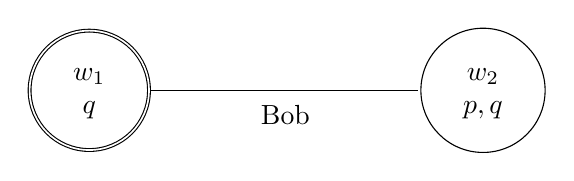
\begin{tikzpicture}
    [every node part/.style={align=center}]
    \node (1) [draw, circle, accepting] at (0, 0){
      \begin{tabular}{c}
        $w_1$ \\
        $q$
      \end{tabular}
    };
    \node (2) [draw, circle] at (5, 0) {
      \begin{tabular}{c}
        $w_2$ \\
        $p, q$
      \end{tabular}
    };

    \draw [-, shorten >= 1pt] (1) -- (2) node [midway, below = 2pt] {Bob};
  \end{tikzpicture}
\end{center}

In this epistemic model, we have two agents, Alice and Bob, and two worlds,
$w_1$ and $w_2$. Alice can distinguish between $w_1$ and $w_2$, and as such has
no lines on the diagram. However Bob cannot, hence the line connecting $w_1$ and
$w_2$. At $w_1$ the proposition $q$ is true, and at $w_2$ propositions $p$ and
$q$ are true. Our ``actual'' world is $w_1$, and as such it is double ringed. 

To show some examples, let's evaluate some formulae on this model.

\begin{itemize}
\item $(\mc{M}, w_1) \models q$ as at $w_1$, $q$ is true.
\item $(\mc{M}, w_1) \models K_{\text{Alice}} q$. To check that this is true, let's
  consider all of the worlds Alice considers possible from $w_1$. The only world
  is $w_1$ itself, and we know from above that $(\mc{M}, w_1) \models q$. Hence
  $K_{\text{Alice}} q$ holds here.
\item $(\mc{M}, w_1) \models \neg K_{\text{Bob}} \left( p \land q \right)$. Now
  let's consider all the worlds that Bob considers possible from $w_1$. This is
  both $w_1$ and $w_2$. But we see that $(\mc{M}, w_1) \not \models (p \land
  q)$, since $(\mc{M}, w_1) \not \models p$. 
\end{itemize}

\subsubsection{Event Models}
\label{sec:Event Models}

Public announcement logic was the first development in epistemic logic to
support information change in epistemic logic, and is described in \cite{PAL}.
However, in public annoucement logic, we may only model truthful, public
communications; but we all know that there are many other types of communication
and events after which some information has changed. An agent may communicate
with another agent in a private phone call, or may be lying to them;
furthermore, we may have some \textit{physical} action, like a coin flip
occuring, after which some knowledge has changed.

To model these more complicated events, we use \textit{event models}. These
treat events in a very similar way to how Kripke models treat worlds; we think
of a set of possible events that can occur, and encode the events that an agent
can tell apart. We give the modern definition of event models, as in
\cite{MalvinThesis}, and \cite{AutomataTechniques}, however these were first
defined in \textbf{Cite 1998 Baltag paper}

Formally, an event model \tmc{E} is a tuple $(E, Q, \pre, \post)$. $E$ is a finite set
of events; $Q$ is a set of relations $Q_i$ for each $i \in Ag$, such that $Q_i
\subseteq E \times E$. As before, we make all relations $Q$ equivalence
relations. $\pre : E \rightarrow \mc{L}(\Lambda) $ is the \textit{precondition
  function}; given an event $e \in E$, it returns to us a formula that must be
true in order for $e$ to occur. $\post : E \times \Lambda \rightarrow
\mc{L}(\Lambda)$ is the \textit{postcondition function}; given an event $e \in
E$ and a proposition $p \in \Lambda$, it returns to us some formula that had to
be true at the prior state $s$ in order for $p$ to be true after event $e$
occurs at $s$. We will later give examples for these two functions.

Updating a Kripke model \tmc{M} with an event model \tmc{E} is gives us another
Kripke model $\mc{M} \times \mc{E} ::= (W', R', V')$, where:

\begin{align*}
  W'   &::= \left\{(w, e) \in W \times E \mid (\mc{M}, w) \models \pre(e)\right\} \\
  R_i' &::= \left\{((w, e), (v, f)) \mid (w, v) \in R_i, (e, f) \in Q_i \right\} \\
  V'(w, e) &::= \left\{ p \in \Lambda \mid (\mc{M}, w) \models \post(e, p) \right\}
\end{align*}

We see that it is the postcondition function that allows for factual change;
that is, the update of what is true at a state given the occurence of some
event.

\bigskip \bigskip \bigskip

As above, we now show some example event models, and show the effects of
updating an epistemic model with an event model.

\begin{figure}
  \centering
  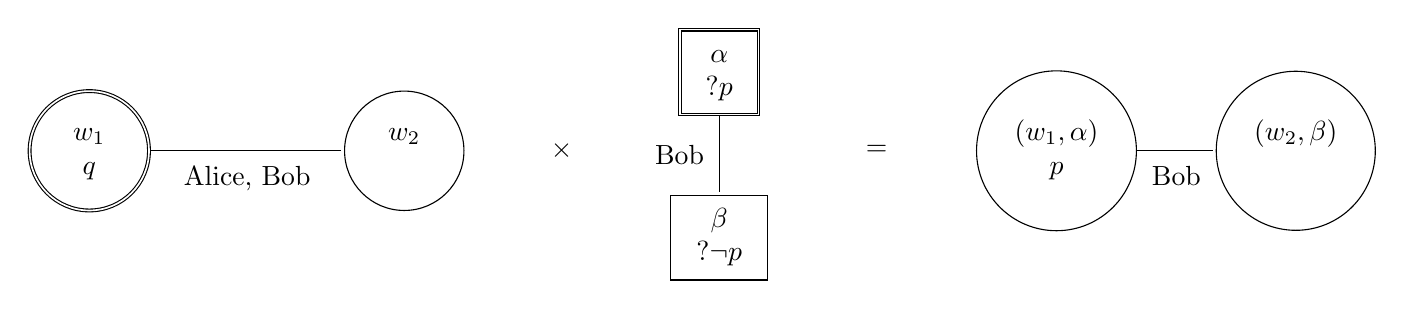
\begin{tikzpicture}
    \node(1) [draw, circle, accepting] at (0, 1) {
      \begin{tabular}{c}
        $w_1$ \\
        $q$
      \end{tabular}
    };

    \node(2) [draw, circle] at (4, 1) {
      \begin{tabular}{c}
        $w_2$ \\
        $$
      \end{tabular}
    };
    \draw[-, shorten >= 1pt] (1) -- (2) node [midway, below = 2pt] {Alice, Bob};

    \node(times) [] at (6, 1) {$\times$};
    
    \node(3) [draw, rectangle, accepting] at (8, 2) {
      \begin{tabular}{c}
        $\alpha$ \\
        $?p$
      \end{tabular}
    };
    \node(4) [draw, rectangle, below = of 3] {
      \begin{tabular}{c}
        $\beta$ \\
        $?\neg p$
      \end{tabular}
    };
    \draw[-, shorten >= 1pt] (3) -- (4) node [midway, left = 2pt] {Bob};

    \node (equals) [] at (10, 1) {$=$};

    \node(5) [draw, circle, right = of equals] {
      \begin{tabular}{c}
        $(w_1, \alpha)$ \\
        $p$
      \end{tabular}
    };
    \node(6) [draw, circle, right = of 5] {
      \begin{tabular}{c}
        $(w_2, \beta)$ \\
        $$
      \end{tabular}
    };

    \draw[-, shorten >= 1pt] (5) -- (6) node [midway, below = 2pt] {Bob};
  \end{tikzpicture}
  \caption{}
  \label{fig:PhDExample}
\end{figure}


In this example, consider two agents, again Alice and Bob. They are waiting in
the same room to receive a letter about Alice's entrance onto a PhD program.
Suddenly the postman arrives, and Bob sees Alice pick up and open a letter with
the University's logo on the front. Alice reads the letter and learns that she
gets the position, but she does not tell Bob the result. Bob sees that Alice now
knows whether she got it, but he does not know if she did get it or not.

Here, $p$ stands for the proposition ``Alice gets the position''. This initial
situation is represented by model \tmc{M}. Both Alice and Bob cannot distinguish
between the worlds where $p$ is true and where $p$ is not true. 

Then the event model \tmc{E} represents the event of Alice reading the letter
from the unviersity. $\alpha$ represents the event of Alice getting the position
and $\beta$ that she doesn't - hence the preconditions are $p$ and $\neg
p$ respectively; that is, $\pre(\alpha) = p$ and $\pre(beta) = \neg p$. Bob
cannot distinguish between either of these events, but Alice can.

Then finally the event model $\mc{M} \times \mc{E}$ represents the situation
in \tmc{M} after the event \tmc{E} has occurred. We can see the epistemic model \tmc{M},
event model \tmc{E} and updated model \tmc{M \times E} in \figref{fig:PhDExample}.

\bigskip

As a second example, consider that Alice and Bob are in a room. There's a coin
on the table with the heads face up - we set this to be represented by the
proposition $p$. Alice and Bob can both see the coin face up. This situation is
modelled by event model \tmc{M}.

Then Bob picks up the coin and flips it in the air. Bob sees the result of this
coin flip, but does not show Alice. We can see the event model and epistemic
model, and their update in \figref{fig:cointoss}.

Our epistemic model has just one state - that is, the state where the coin is on
the table face up. Both Alice and Bob can see the coin, and as such they both
know that $p$ holds. Then our event model has two events; $\alpha$, in which the
coin lands face-up, and $\beta$, in which the coin lands face-down. Bob can
distinguish between these two events as he can see the result of the coin toss,
but Alice cannot, because she does not see it. In the former $p$ is set to true,
and in the latter $p$ is set to false. Hence in the epistemic model $(\mc{M}
\times \mc{E})$ we have two states; that in which the coin landed face-up and
that in which the coin landed face-down.

\begin{figure}[h]
  \centering
  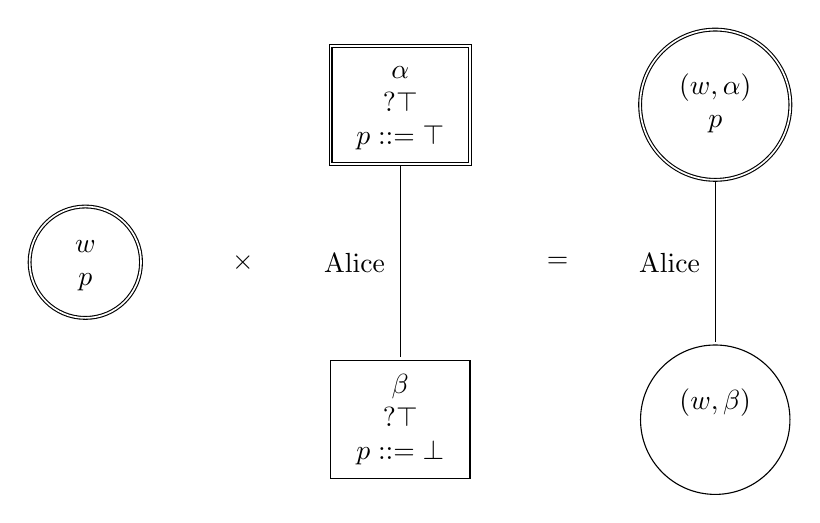
\begin{tikzpicture}
    [every node part/.style={align=center}]
    \node (0) [draw, circle, accepting] at (0, 2) {
      \begin{tabular}{c}
        $w$ \\
        $p$
      \end{tabular}
    };
    \node (1) [draw, rectangle, accepting] at (4, 4) {
      \begin{tabular}{c}
        $\alpha$ \\
        $?\top$ \\
        $p ::= \top$
      \end{tabular}
    };

    \node (times) at (2, 2) {$\times$};
    \node (2) [draw, rectangle] at (4, 0) {
      \begin{tabular}{c}
        $\beta$ \\
        $?\top$ \\
        $p ::= \bot$
      \end{tabular}
    };

    \node(3) [draw, circle, accepting] at (8, 4) {
      \begin{tabular}{c}
        $(w, \alpha)$ \\
        $p$
      \end{tabular}
    };

    \node (equals) at (6, 2) {$=$};
    
    \node(4) [draw, circle] at (8, 0) {
      \begin{tabular}{c}
        $(w, \beta)$\\
        $$
      \end{tabular}
    };

    \draw [-, shorten >= 1pt] (1) -- (2) node [midway, left = 2pt] {Alice};
    \draw [-, shorten >= 1pt] (3) -- (4) node [midway, left = 2pt] {Alice};
  \end{tikzpicture}
  \label{fig:cointoss}
  \caption{An event model and epistemic model for the coin toss example, and the
  updated event model. }
\end{figure}
    

\subsection{The Gossip Problem}

Gossip is a procedure for spreading secrets around a group of agents, where the
agents are commonly displayed as nodes in a graph and the ability of one agent
to contact another displayed as an edge between two nodes. Gossip was first put
forward in \cite{Tijdeman:1971}, where the network is a complete graph; all
agents can contact one another. One question here was to find how many calls are
needed for every agent to learn the secret of every other agent. We will
henceforth describe an agent knowing the secret of every other agent as this
agent being an \textit{expert}. It was quickly proved (\cite{TelephoneDisease},
\cite{GandT}) that this number, for a network where the number of agents $n$ is
greater than 4, is $2n - 4$.
 
\subsubsection{Dynamic Gossip}

Dynamic Gossip is a variant of the classical gossip problem, in which we start
off with an incomplete graph, representing the fact that the agents have only
the phone numbers of some of the other agents. In this case, when two agents
talk on the phone, they also exchange all of the phone numbers that they know, as
well as the secrets that they know.

\subsubsection{Protocols}
\label{sec:Protocols}

The gossip problem, as we have mentioned so far, can rely on some central
scheduler to tell the agents what call to make, and lets them know when to stop.
However in distributed computing, methods that do not require this central
authority are desirable. In such a situation, the agents need to have some form
of rules to follow to decide how to behave and who to call next. This is the
motivation for a \textit{gossip protocol}, which are short conditions that must
be fulfilled in order for an agent to make a specific call. These protocols were
first proposed in \cite{EPfDG}, \cite{KnowledgeandGossip}, and some exemplar
ones are:

\begin{itemize}
\item \textsf{ANY} - If $x$ knows the phone number of $y$, $x$ may call $y$.
\item \textsf{LNS} - If $x$ knows the phone number of $y$ and $x$ does not
    know the secret of $y$, then $x$ may call $y$.
\end{itemize}

In this thesis, we do not study the distributed gossip problem; rather, a
version with a central authority that surveys the network topology and then
decides which agent is allowed to make a call, and also who they will call.
However, these protocols do still have use for us. \textsf{ANY} allows for
infinite call sequences - for example, one where agent $a$ just repeatedly calls
$b$, whereas all of the call sequences induced by \textsf{LNS} are of finite
length. In the long run this does not really matter; both \textsf{ANY} and
\textsf{LNS} have runtime expected execution length in $O(n \log n)$
(\cite{DynamicGossip}), yet in our implementation tests performed with
\textsf{LNS} took considerably less time than \textsf{ANY}. For this pragmatic
reason \textsf{LNS} is often used in this thesis.

It should also be noted that there are certain classes of graphs for which
\textsf{LNS} cannot induce a successful call sequence, yet \textsf{ANY} can
(\cite{DynamicGossip}). However, this thesis does not investigate this topic,
and as such this will no longer be mentioned. 

\subsubsection{Formalisation}

We now go on to formalise some of the ideas mentioned so far in this section.
The definitions of gossip graphs are classic and can be found in all of the
related literature (e.g. \cite{DynamicGossip}, \cite{MalvinThesis})

\bigskip

We formally denote a gossip graph \tmc{G} with a triple $(A, N, S)$. $A$ is a
finite set of agents in the graph; $N \subseteq A \times A$ is a set of ordered
pairs of agents such that $(u, v) \in N$ (or $Nuv$) iff $u$ knows the phone
number of $v$. $S \subseteq A \times A$ is a set of ordered pairs of agnets such
that $(u, v) \in S$ (or $Suv$) iff $u$ knows the \textit{secret} of $v$.

\begin{figure}[h]
  \centering
  \begin{subfigure}[b]{0.4\textwidth}
    \centering
    \begin{tikzpicture}
      \node (a) [] at (0, 1) {$a$};
      \node (b) [] at (2, 0) {$b$};
      \node (c) [] at (3, 2) {$c$};

      \draw [<->, dashed] (a) -- (b);
      \draw [->, dashed] (b) -- (c);
    \end{tikzpicture}
    \caption{An exemplar gossip graph.}
    \label{fig:GossipSize3}
  \end{subfigure}%
  ~
  \begin{subfigure}[b]{0.4\textwidth}
      \centering
    \begin{tikzpicture}
      \node (a) [draw, rounded rectangle, accepting] {
        \begin{tikzpicture}
          \node (a) [] at (0, 1) {$a$};
          \node (b) [] at (2, 0) {$b$};
          \node (c) [] at (3, 2) {$c$};

          \draw [<->, dashed] (a) -- (b);
          \draw [->, dashed] (b) -- (c);
        \end{tikzpicture}
      };
    \end{tikzpicture}
    \caption{A Kripke model $\mc{G}$ for a Gossip State}
    \label{fig:KripkeGossip}
  \end{subfigure}
  \caption{}
  \label{fig:Gossip2Kripke}
\end{figure}


We also have that for all gossip graphs, for any agent $a$, $(a, a) \in N$ and $(a, a)
 \in S$, expressing that any agent always knows their own phone number and
 secret.

\bigskip
 
We can use the notation above to formally describe a gossip graph. For instance,
the gossip graph that we can see in \figref{fig:GossipSize3} can be expressed as
the triple $\mc{G} = (\left\{ a, b, c \right\},$ $ \left\{ (a, a), (a, b), (b, a), (b,
  b), (b, c), (c, c) \right\},$ $ \left\{ (a, a), (b, b), (c, c) \right\})$.
However given that we have the proprety described above, we can represent this
as the more terse $\mc{G} = (\left\{ a, b, c \right\},$ $ \left\{ (a, b), (b,
  a), (b, c)
\right\}, $ $ \left\{ \right\})$

\bigskip

One might ask how gossip fits into the picture we drew above of Kripke models
and event models. We give a way to generically define Kripke models and event
models for an arbitrary gossip graph $\mc{G} = (A, N, S)$. A Kripke model for a
graph \tmc{G} uses the set of propositions $\{N_{ij} \mid i \in A, j \in A\}
\cup \{S_{ij} \mid i \in A, j \in A\}$. The Kripke model for a graph \tmc{G} has
just one state, $q$, which is the state that models the graph. We define
$\mc{M_G} = (W, R, V)$ where $W = \left\{ q \right\}$, $R_i = \left\{ (q, q)
\right\}$ for every agent $i \in A$, and $V(q) = \{N _{ij} \mid (i, j) \in N\}
\cup \{S_{ij} \mid (i, j) \in S\}$. An example of this is just in
\figref{fig:Gossip2Kripke}; we see that the Kripke model for the graph is not
particularly complicated. 

An event model can also be produced in a similar way. We make an event model
$\mc{E} = (E, P, \pre, \post)$, where

\begin{itemize}
\item $E = \{ij \mid i \in A, j \in A, i \not = j\}$. Our set of events is the
  calls between agents, however an agent cannot call themself. 
\item $P_i = \left\{(jk, j'k') \mid j, k, j', k' \in A, i \not \in \{j, k, j',
    k'\}\right\} \cup \left\{ (ij, ij) \mid j \in A\right\} \cup \left\{ (ji,
    ji) \mid j \in A \right\}$, for every $i \in A$. We can read this as agent
  $i$ cannot distinguish between a call that it is not a part of; hence the
  former part of the definition. The later two sets say that agent $i$ does not
  confuse a call that it's a part of with any other call. 
\item $\pre(ij) = N_{ij}$. By this we mean that the precondition for a call from
  agent $i$ to $j$ is that $i$ knows the phone number of $j$. \\
  It is here that we
  can add in protocols from \secref{sec:Protocols}; for instance, in an event
  model where we follow the protocol \textsf{LNS}, we add the condition $\neg
  S_{ij}$ to the precondition; hence $\pre_{\textsf{LNS}}(ij) = N_{ij} \land
  \neg S_{ij}$.
\item $\post(ij, N_{nm}) = \left\{ \begin{array}{ll}
                                     N_{im} \lor N_{jm} & \text{if $n == i$ or $n ==
                                                     j$} \\
                                     N_{nm} & \text{otherwise} 
                                   \end{array}
                           \right.$ \\
$\post(ij, S_{nm}) = \left\{ \begin{array}{ll}
                                     S_{im} \lor S_{jm} & \text{if $n == i$ or $n ==
                                                     j$} \\
                                     S_{nm} & \text{otherwise} 
                                   \end{array}
                           \right.$ \\
 This states that if a call occurs, then for an agent $n$ to know the number of
 an agent $m$, either $n$ was a part of the call and $n$ either knew the number
 of $m$ before or learned it from speaking to the other agent in the call, or
 $n$ was not a member of the call and knew the number of $m$ anyway. The same
 goes for secrets. 
\end{itemize}

We now give the event model for the graph \figref{fig:GossipGraph3} as an
example. 

\begin{figure}[h]
  \centering
  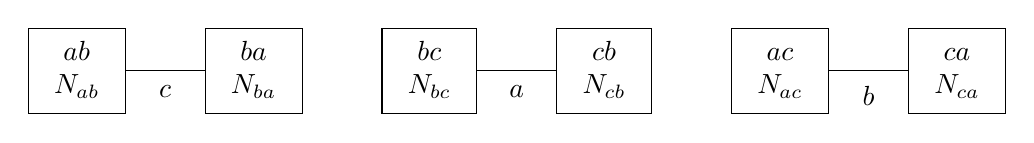
\begin{tikzpicture} [every node/.style={draw,rectangle}]
    \node (ab) [] {
      \begin{tabular}{c}
        $ab$ \\
        $N_{ab}$ 
      \end{tabular}
    };
    \node (ba) [right = of ab] {
      \begin{tabular}{c}
        $ba$ \\
        $N_{ba}$ 
      \end{tabular}
    };
    \node (bc) [right = of ba] {
      \begin{tabular}{c}
        $bc$ \\
        $N_{bc}$ 
      \end{tabular}
    };
    \node (cb) [right = of bc] {
      \begin{tabular}{c}
        $cb$ \\
        $N_{cb}$ 
      \end{tabular}
    };
    \node (ac) [right = of cb] {
      \begin{tabular}{c}
        $ac$ \\
        $N_{ac}$ 
      \end{tabular}
    };
    \node (ca) [right = of ac] {
      \begin{tabular}{c}
        $ca$ \\
        $N_{ca}$ 
      \end{tabular}
    };
    
    \draw [-] (ab) -- (ba) node [draw=none, midway, below = 2pt] {$c$};
    \draw [-] (bc) -- (cb) node [draw=none, midway, below = 2pt] {$a$};
    \draw [-] (ca) -- (ac) node [draw=none, midway, below = 2pt] {$b$};
  \end{tikzpicture}
  \caption{An Event model $\mc{E_G}$ for the calls associated with \figref{fig:GossipSize3}.}
  \label{fig:GossipEvMo}
\end{figure}

\begin{figure}
  \centering
  \begin{tikzpicture}
    \node (0) [draw, rounded rectangle] at (0, 4) {
      \begin{tabular}{c}
        $(w, ab)$ \\
        \begin{tikzpicture}
          \node (a) [] at (0, 1) {$a$};
          \node (b) [] at (2, 0) {$b$};
          \node (c) [] at (3, 2) {$c$};

          \draw [<->] (a) -- (b);
          \draw [->, dashed] (a) -- (c);
          \draw [->, dashed] (b) -- (c);
        \end{tikzpicture} 
      \end{tabular}
    };
    \node (1) [draw, rounded rectangle] at (8, 4) {
      \begin{tabular}{c}
        $(w, ba)$ \\
        \begin{tikzpicture}
          \node (a) [] at (0, 1) {$a$};
          \node (b) [] at (2, 0) {$b$};
          \node (c) [] at (3, 2) {$c$};

          \draw [<->] (a) -- (b);
          \draw [->, dashed] (a) -- (c);
          \draw [->, dashed] (b) -- (c);
        \end{tikzpicture} 
      \end{tabular}
    };
    \node (2) [draw, rounded rectangle] at (4, 0) {
      \begin{tabular}{c}
        $(w, bc)$ \\
        \begin{tikzpicture}
          \node (a) [] at (0, 1) {$a$};
          \node (b) [] at (2, 0) {$b$};
          \node (c) [] at (3, 2) {$c$};

          \draw [<->, dashed] (a) -- (b);
          \draw [<->] (b) -- (c);
          \draw [->, dashed] (c) -- (a);
        \end{tikzpicture} 
      \end{tabular}
    };

    \draw [-] (0) -- (1) node [midway, above = 2 pt] {$c$};
  \end{tikzpicture}
  \caption{The Kripke model $\mc{G} \times \mc{E_G}$.}
  \label{fig:UpdatedGossip}
\end{figure}

In \figref{fig:UpdatedGossip} we can see the result of updating the Kripke model
\tmc{G} with the event model \tmc{E_G}. We see that the call $cb$ does not have
a corresponding state; its precondition was not satisfied by any of the states
in \tmc{G}. Also note that the states $(w, ab)$ and $(w, ba)$ are
indistinguishable to $c$; this is because $c$ cannot distinguish between calls
$ab$ and $ba$ as $c$ is not included in it. Also note that the two states $(w,
ab)$ and $(w, ba)$ have the exact same graph representing them\footnote{We
  revisit this idea of gossip graphs with three agents being ``boring'' again
  later. This ``boring''-ness comes from the fact that calls $ab$ and $ba$ are
  essentially the same thing.}; in the future we
will not make this distinction. In the implementation a state is represented
\textit{just by the propositions that are true at it}; in our case, this is the
graph. 

\subsection{Planning}

Automated planning is the process of computing which set of events must occur to
take a system from some given initial state to some successful state. Such a
system is defined as a triple $\Sigma = (S, A, \gamma)$, where:

\begin{itemize}
\item $S$ is some set of states;
\item $A$ is some set of \textit{actions};
\item $\gamma : S \times A \hookrightarrow S$ is a state-transition function. It
  is partial; for $s \in S, a \in A$, either $\gamma(s, a) \in S$ or it is
  undefined. 
\end{itemize}

Then an instance of the planning problem is a triple $(\Sigma, s_i, S_g)$,
where;

\begin{itemize}
\item $\Sigma$ is a planning system;
\item $s_i \in S$ is some initial state;
\item $S_g \subseteq S$ is some set of goal states.  
\end{itemize}

A \textit{solution} to the planning problem is some ordered set of actions
${a_0, a_1, \ldots, a_n}$ such that $\gamma(\gamma(\ldots \gamma(s_0, a_0)
\ldots ,a_{n-1}) ,a_n) \in S_g$. 

Note that we call a planning problem \textit{multi-agent} if the number of
agents in the system is greater than 1, and \textit{single-agent} if the number
of agents is equal to 1. 

\subsubsection{Epistemic Planning}

The dynamic epistemic logic community has recently been investigating a special case
of planning, namely \textit{epistemic} planning (\cite{BolanderEP},
\cite{UndecidabilityEP}). This is planning where we may have some initial
epistemic state (e.g. agent $a$ knows $\phi$), some actions that update these
epistemic states, and some accepting epistemic state (e.g. agent $b$ knows
$\psi$). It is not hard to see how this can be applied to the gossip problem.

We give a formal definition of the epistemic planning problem that slightly
differs from convention, however with this definition and those from the
literature are equivalent. Then the epistemic planning problem is as follows;
given a pointed epistemic model $(\mc{M}, w)$ and an event model $\mc{E}$, and
some goal formula $\phi$, find some set of events ${e_1, e_2, \ldots, e_n}$ such
that $(\mc{M}, w) \otimes (\mc{E}, e_1) \otimes \ldots \otimes (\mc{E}, e_n)
\models \phi$. The \textit{propositional epistemic planning problem} is the
restriction of the epistemic planning problem to event models with pre- and
post-condition functions whose codomains are in the propositional fragment of
\tmc{L}; that is, they do not contain the modal operator $K$. These event models
are what we call propositional event models.

It is proven in \cite{BolanderEP} that the multi-agent epistemic planning
problem is undecidable for an aribtrary system. However, placing certain
restrictions on the system used yields decidability (\cite{DecidabilityEp},
\cite{AutomataTechniques}). One particularly important result is that the
propositional epistemic planning problem is decidable; indeed, it is this result
that this thesis relies on. 

\bigskip \bigskip \bigskip

In this thesis, we focus on solving the epistemic planning problem by means of
the automata constructions described in \cite{AutomataTechniques}. These
methods, and the resulting piece of software associated with this thesis, are
unique in that they will work for any epistemic model and (propositional) event
model. This unfortunately means that we cannot plan for situations like muddy
children or drinking logicians (\cite{DEMO-S5}) as they require epistemic pre-
or post-conditions. 


\subsection{Existing Tools}

We now give an overview of existing software in the realm of model checking or
planning for epistemic systems.

\subsubsection{DEMO-S5}

DEMO-S5 (\cite{DEMO-S5}) is a model checker for epistemic models, limited to
$S5$ models. It is also limited in that it only supports events that are either
public announcements (e.g. an agent telling every other agent some statement) or
publicly observable factual change (e.g. the flip of a coin, where the result is
seen by every agent).

It performs the task of model checking by taking an epistemic model and a
formula representing either the announcement or the fact that changed, and
updating the model with the event represented by the formula. The definition of
the update used is very similar to the update of an epistemic model with an
event model as defined in Section \ref{sec:Event Models}. The given events are
applied, and at this point we check if we're in a successful state or not.

\bigskip

Unfortunately we cannot use this to model check a gossip problem, as events in
the gossip problem are neither of these; they are private one-to-one
communications. Furthermore, the software is incapable of planning; simply
checking. Despite this, the software was incredibly useful in our project in
aiding the understanding of epistemic and event models. Indeed, the
formalisation of epistemic and event models demonstrated here was used in the
code associated with this thesis.

\subsubsection{Gossip}

\cite{GithubGossip} is another model checker, however now for strictly the
gossip problem. This program has a significant advantage over the other two
pieces of software; namely that it is capable of planning. It does this by
generating all of the possible sequences of calls on the graph and then checking
which of these are successful (i.e., after execution of all of the calls the
graph is in some successful state) and which are not. It also has further
capabilities for studying protocols deeply, however these are not relevant to
our thesis.

Although the methods used within this software are very different to the ones
used in our implementation, this system proved to be very useful for testing
purposes, due to its simplicity of use. The results returned by our software
during testing were verified using this system. Further elaboration on this will
be given in the evaluation section of this thesis.

One limitation of this system is that is may only handle gossip states, and not
generic epistemic models. Also limiting is that it enumerates all possible call
sequences from the initial state; we are only interested in successful ones.
This means that we have the possibility of lots of wasted computation if we need
to validate lots of unsuccessful paths before we get to a successful one. 

\subsubsection{SMCDEL}

SMCDEL is the most sophisticated of the three pieces of software. A technical
report is given in \cite{SMCDEL}, whilst a lot of the underlying theory is in
\cite{MalvinThesis}. The main difference is that it uses \textit{symbolic model
  checking}, a method put forward in \cite{SymbolicModelChecking}. This gives a
much more efficient implementation \textbf{why}?, as can be seen in the
Chapter 4 of \cite{MalvinThesis}.

This software is capable of efficiently model checking all classes of epistemic
models, and also has capacity for planning; however this side of the program is
not well-displayed, and it is unclear precisely how to use it. Furthermore, due
to a reasonably unpleasant interface we choose not to use this software for
benchmarking and instead use the simpler \cite{GithubGossip}. 

\subsection{Uniform Strategies}

In this thesis, we use a lot of ideas from \cite{AutomataTechniques}. This paper
puts forward a method for epistemic planning, through use of automata
representing states of the model and events in the event model as the states and
transitions respectively. This then references a process in
\cite{UniformStrategies} for the creation of an automata which has a set of the
other indistinguishable states baked into the states of the automata. This is a
very useful method for our context, as it means that we can evaluate formulas of
the form $K_a \phi$ \textit{positionally}; that is, we need only to look at the
state to be able to evaluate the formula. We often want to reach states in the
gossip problem which satisfy the property ``everyone knows that everyone knows
everyone's secret''. This is formalised as $\forall a, i, j \in Ag, K_a (S
_{ij})$.

This method is much more practical than the alternative, which is to check our current
state then compute the possible call sequences that are indistinguishable from
our current one, and then go and check there too, and so on.

The process in \cite{UniformStrategies} is very verbose and is beyond the scope
of this thesis; however, in order to illustrate the fact that our algorithm is a
special case of the process, we give a brief introduction to the process and its
theory. We slightly change some of the definitions to lend itself better to our
scenario. The setting is game theory; hence the frequent references to plays and
strategies.

\subsubsection{Game Arenas}

A game with \textit{imperfect information} is a game in which the players have
some uncertainty concerning hte current configuration of the game (for example
Poker; a player does not know which cards are in the other players' hands). A
player in such a game cannot plan to play differently in a situation she cannot
distinguish; hence we have to define her strategy \textit{uniformly} across
situations she cannot distinguish. 

We consider two-player turn-based games played on a some graph, where the
vertices are labelled with propositions. These propositions hold some useful
information about the state; it could be what people know about it, or some fact
about the environment the player is in and so on. This set of propositions will
be referred to as $AP$. 

Then a game arena is a structure $\mc{G} = (V, E, v_I, l)$ where $V = V_1 \uplus
V_2$ \footnote{We use $\uplus$ here to indicate that this is a partition} is a
set of positions split between those of Player 1 ($V_1$) and those of Player 2
($V_2$). $E \subseteq (V_1 \times V_2) \cup (V_2 \times V_1)$ is the set of
edges, $v_I \in V$ is the initial position and $l : V \rightarrow \mc{P}(AP)$ is
a valuation function, which maps each position to the finite set of propositions
that are true at it.

\subsubsection{Transducers}
\label{subsec:Transducers}

We give a quick recap of transducers, as they are used heavily in the next two
sections. A transducer is like a nondeterministic finite automaton with two
tapes; an \textit{input} tape and an \textit{output} tape. The transducer reads
an input finite wood on its input and writes a finite word on its output tape.
Hence a transducer defines a binary relation. Relations recognised by a
transducer are called \textit{regular} or \textit{rational} relations. 

A transducer is a 6-tuple $T = (Q, \Sigma, \Gamma, I, F, \Delta)$, where $Q$ is
a finite set of states, $\Sigma$ is the input alphabet, $\Gamma$ is the output
alphabet, $I \subseteq Q$ is a finite set of initial states, $F \subseteq Q$ is
a finite set of final states, and $\Delta \subseteq Q \times \left( \Sigma \cup
  \{\epsilon\} \right) \times \left( \Gamma \cup \{\epsilon\} \right) \times Q$
is the transition function.

$(q, a, b, q') \in \Delta$ means that the transducer can move from state $q$ to
state $q'$ by reading $a$ from the input tape and writing $b$ to the output
tape. We will use this notation throughout, however this is equivalent to saying
that $\Delta(q, a) = (b, q')$. Note that transducers are, in this thesis,
nondeterministic; hence if $\Delta = \left\{ (q, e, f, p), (q, e, g, r)
\right\}$ then $\Delta(q, e) = \left\{ (f, p), (g, r) \right\}$.

Then we can define the extended transition relation $\Delta^\ast$ as the
smallest relation satisfying:

\begin{itemize}
\item for all $q \in Q$, $(q, \epsilon, \epsilon, q) \in \Delta^\ast$
\item if $(q, w, w', q') \in \Delta^\ast$ and $(q', a, b, q'') \in \Delta$, then
  $(q, w . a, w' . b, q'') \in \Delta^\ast$
  
\end{itemize}

We can see $\Delta^\ast$ as the transitive closure of $\Delta$. We abbreviate
$(q, w, w', q') \in \Delta^\ast$ to $q \rsarrow_{w \mid w'} q'$ in the rest of
this section.

Finally, we say that the relation recognised by some transducer $T$ is

\begin{align*}
  [T] ::= \left\{ (w, w') \mid w \in \Sigma^\ast, w' \in \Gamma^\ast, \exists q_F \in F, \exists q_i \in I, q_i \rsarrow_{w \mid w'} q_F \right\}
\end{align*}

\subsubsection{The Powerset Arena}
\label{sec:PowersetArenaena}

In games with imperfect information, the information set of a player after a
certain play is the set of positions she may possibly be in, consistent with
what she has observed\footnote{For instance in a game of poker with one deck of cards, a
player may have no idea what the other players have in their hands except that
they know they do not have the cards the player has in their own hands, nor the
cards face-up on the table.}. We can define a similar notion in our setting, and
we show that this is sufficient to build a powerset arena in which formulas of
the form $K_a \phi$, where $\phi$ is propositional, can be evaluated positionally. 

For an arena \tmc{G} and a transducer $T$ over finite sequences of events $e_i \in
E$, we construct this automata $\widehat{\mc{G}}$ in which we can evaluate
formulas of the form $K_i \phi$... 

Our new information set after a move occurs cannot be computed knowing only the
previous information set and the new position; we need to simulate the
nondeterministic execution of $T$, taking as input the sequence of positions
played and writing as output the related plays. Precisely, we need two things;
the set of states the transducer may be in after reading the sequence of
positions played so far, and for each of these states the set of possible last
positions written on the output tape. We need only remember the last letter and
not the whole tape because the information set we aim to compute is just the set
of the last positions of related plays.

Then our positions are of the form $(v, S, Last)$, where $v \in V$, $S \subseteq
Q$, where $Q$ is the set of states in the transducer and $S$ is the set of
possible current states of $T$, and $Last : S -> \mc{P}(V)$\footnote{It may be
  more helpful to think of this as something a bit more tangible than a
  function, e.g. a list of tuples $(S, [P])$} associates to a state $q \in S$
the set of the possible last positions on the output tape fo $T$ if the current
state is $q$. The transitions in this arena follow those in \tmc{G}, except we
now maintain the additional information about the configuration of the
transducer.

To construct the initial position $\widehat{v_I} = (v_I, S_I, Last_I) \in
\widehat{\mc{G}}$, we need to simulate the execution of $T$ starting from its
initial state and reading $v_I$. To do this, we introduce an artificial position
$\widehat{v_{-1}} = (v_{-1}, S_{-1}, Last_{-1})$, where $v_{-1} \not \in V$ is
some fresh position, $S_{-1} = \{q_i\}$ where $q_i$ is the initial state of the
transducer because before starting the transducer is in its initial state, and
$Last_{-1} (q_i) = \emptyset$ because we have nothing written on the output
tape.  

\bigskip

We now come onto defining \tmc{G}. Let $\mc{G} = (V, E, v_I, l)$ be an arena and
$T = (Q, V, q_i, Q_F, \Delta)$ be an FST. Then we define the arena
$\widehat{\mc{G}} = (\widehat{V}, \widehat{E}, \widehat{v_I}, \widehat{l})$ as:

\begin{itemize}
\item $\widehat{V} = V \times \mc{P}(Q) \times (Q \rightarrow \mc{P}(V))$
\item $(u, S, Last) \widehat{\rightarrow} (v, S', Last')$ if
  \begin{itemize}
  \item $u = v_{-1} \text{ and } v = v_I, \text{ or } u \rightarrow v$,
  \item $S' = \left\{q' \mid \exists q \in S, \exists \lambda' \in V^\ast, q
      \rsarrow_{v \mid \lambda'} q' \right\}$ and
  \item $Last' (q') = \left\{ v' \mid \exists q \in S, \exists \lambda' \in
      V^\ast, q \rsarrow_{v \mid \lambda' \circ v'} q', \text{ or } q \rsarrow_{v \mid
        \epsilon} q' \text{ and } v' \in Last(q) \right\}$
  \end{itemize}
\item $\widehat{v_I}$ is the only $\widehat{v} \in \widehat{V}$ such that
  $\widehat{v}_{-1} \widehat{\rightarrow} \widehat{v}$.
\item $\widehat{l}(\widehat{v}) = l (v)$ if $\widehat{v}= (v, S, Last)$. 
\end{itemize}

The definition of transitons is quite complicated, and as such we give a high-level
explanation of it. Regarding the definition of the transitions,
the first point means that our transitions in $\widehat{E}$ follow those in $E$,
except for the transition leaving $\widehat{v_{-1}}$, which we use to define
$\widehat{v_I}$. 

The second point expresses that when we move from $u$ to $v$ in \tmc{G}, we give
$v$ as input to the transducer. Then the set of states that we can be in, that
is, $S'$, is the set of states that can be reached from some previous possible
state in $q \in S$ by reading $v$ on the input tape and outputting some sequence
$\lambda'$.

Finally, the third point expresses that if some position $v'$ is at the end of
the output tape after the transducer reads $v$ and reaches $q$, then this is either
because while reading $v$ the last letter it wrote is $v'$, or it wrote nothing
and $v'$ was already at the end of the output tape before reading $v$. 

Finally, we say that $\widehat{v}_I$ is the only successor of
$\widehat{v}_{-1}$, and that the valuation of a position in the powerset arena
is the valuation of the underlying position in the original arena. 

\subsubsection{Lifting Transducers}

We can keep on repeating this process, creating a power-powerset arena
$\widehat{\widehat{G}}$. However we first need to lift our transducer $T$ where
$[T] \subseteq Plays_\ast \times Plays_\ast$ to a transducer $\widehat{T}$ where
$[\widehat{T}] \subseteq \widehat{Plays_\ast} \times \widehat{Plays_\ast}$.

We write $T\downarrow$ for the transducer that computers the bijective function
$f$ that maps a play $\widehat{p} \in \wh{Plays_\ast}$ to the underlying play $p
\in Player_\ast$, and $T\uparrow$ for the deterministic transducer that computes
$f^{-1}$. Both can be easily constructed from our powerset arena $\wh{G}$.

Then the lift of a transducer $T$ is $\wh{T} = T\downarrow \circ T \circ
T\uparrow$.

Once we have the transducer $\wh{T}$, we can repeat the process in Section
\ref{sec:PowersetArena} with $\wh{G}$ to get $\wh{\wh{G}}$, and so on ad
infinitum. $\wh{\wh{G}}$ would allow us to positionally check formulae of the
form $K_i K_j \phi$.

\newpage

\section{Algorithm}

\subsection{Introduction}

In this section, we formalise the algorithm that we use to solve the
propostional epistemic planning problem. We see this as a meaningful
contribution of the thesis; there is no existing, clear implementation of this
in the literature.

We first give a rough explanation of the process, before getting into the
details of the process later in this chapter.

As input, we receive an epistemic model \tmc{M}, an event model \tmc{E}, and
some formula $\phi \in \mc{L}(\Lambda)$, for some set of propositions $\Lambda$.
First, we construct an automata called \mestar, by simulating the repeated
application of \tmc{E} on \tmc{M}. This lets us easily traverse the space of
possible states we could be in, after applying the events in \tmc{E} to the
model \tmc{M}.

For the next step, we need to consider the shape of the formula $\phi$. If it
does not include a knowledge modality $K_i$ then we proceed to the next stage.
If it does, then we need to perform the process detailed in Section
\ref{sec:PowersetAdapted}, where the transducer $\mc{T}_i$ used is the
transducer relating the events that are indistinguishable to agent $i$. This is
a powerful procedure that brings the information regarding the states that are
indistinguishable to the agent $i$ into the state we are currently in. Then, in
order to check if a formula of the form $K_i \phi$ is true, we just need to
check that $\phi$ holds at all of the states that are indistinguishable from our
current one. We can now do this in a very straightforward manner, given that the
information regarding the states we could be in is now baked-into the state.

We repeat the process in Section \ref{sec:PowersetAdapted} each time we
encounter a $K$ modality \footnote{Note that in a situation where we have a
  formula $K_a K_a \phi$ we do not need to build another powerset automata as in
  an \textsf{S5} model, $KK \ldots KK = K$ (\cite{ModalLogic}). However, for a
  formula $K_a K_b \phi$ we do; this is because we can see $K_i$ and $K_j$ as
  being different modalities for different agents $i$ and $j$.}; in cases where
we have a conjunction or negation where one of the formulas
included is a knowledge-based formula, then we perform intersection and
complement of the resulting automata. This is a very pleasing result and is a
great display of why finite-state automata are so well suited to this area.

Finally, once we have finished building automata we perform breadth-first search
on the resulting machine. At this point, we have an automata in which formulae
of the same shape \footnote{By shape, we mean that the propositions in the
  formula may be anything in $\mc{L}_P(\Lambda)$, as long as the knowledge
  modalities, conjunctions and negations remain in place} as $\phi$ can be
evaluated positionally. Then we set the states which satisfy $\phi$ to
be the successful states. We can now perform breadth-first search on the
resulting automata to find the shortest path to a successful state.

\bigskip \bigskip \bigskip

With this all in mind, we now move into the implementation details of the
system. 

\subsection{\mestar}
\label{subsec:mestar}

Put forward in \cite{AutomataTechniques}, \mestar is a structure we use to
represent the states that can be reached given an epistemic model \tmc{M} and an
event model \tmc{E}. It consists of an automata \tmc{A_D} and a set of
transducers $\mc{T} = \left\{ \mc{T}_i \mid i \in A \right\}$. The automata
\tmc{A_D} holds the information about the set of possible states that can be
reached using \tmc{M} and \tmc{E}, whilst $\mc{T}_i$ relates pairs of events
that agent $i$ cannot distinguish between. We revisit \tmc{T} later in this
section; for now, we address \tmc{A_D}.

\bigskip

\tmc{A_D} represents the application of some event model \tmc{E} onto an epistemic
model \tmc{M} infinitely. Consider that $\mc{ME}^0$ represents $\mc{M}$,
$\mc{ME}^1$ would be $\mc{M} \times \mc{E}$, and $\mc{ME}^2$ represents $\mc{M}
\times \mc{E} \times \mc{E}$, and so on and so forth. Then we define \mestar as

\begin{equation*}
  \mc{ME}^\ast = \bigcup_{n \geq 0} \mc{ME}^n
\end{equation*}

One might wonder how we can reason about this; it's a seemingly infinite
structure. The key thing to realise is that our states in \mestar are indexed by
the set of propositions that hold true at the state. For instance,
\figref{fig:KripkeGossip} would be represented by the state $q_{\{N_{aa},
  N_{ab}, N_{ba}, N_{ba}, N_{bc}, N_{cc}\}}$. Recall that the set of propositions that
our epistemic model ranges over has to be finite; consequently, our set of
states is finite\footnote{Indeed, we know the exact size of our set of states in
\mestar, which is $2^{|\Lambda|}$.}. The transitions in \mestar are exactly
those from states in \tmc{M} from \tmc{E}. It becomes very clear to see how this
works once we inspect the definition of \mestar. 

% We can picture \mestar as having layers, where each node in a layer $\mc{ME}^n$ has taken
% exactly $n$ events to arrive there.

% \begin{center}
%   \begin{tikzpicture}[every node part/.style={align=center}]
%     \node(0) [draw, rounded rectangle] at (0, 4) {States in $\mc{ME}^0$};
%     \node(1) [draw, rounded rectangle] at (0, 2) {States in $\mc{ME}^1$};
%     \node(2) [draw, rounded rectangle] at (0, 0) {States in $\mc{ME}^2$};
%     \node(3) at (0, -2) {\ldots};

%     \draw[->, shorten >= 1pt] (0) -- (1) node [midway, left = 3pt] {Calls in \tmc{E}};
%     \draw[->, shorten >= 1pt] (1) -- (2) node [midway, left = 3pt] {Calls in \tmc{E}};
%     \draw[->, shorten >= 1pt] (2) -- (3) node [midway, left = 3pt] {Calls in \tmc{E}};
%   \end{tikzpicture}
% \end{center}

% \mestar consists of an automaton $A_{\mc{D}}$ and a set of transducers $\left\{
% \mc{T}_i \mid i \in A \right\}$. $A_{\mc{D}}$ represents the states in our
% epistemic model \tmc{M} and the transitions between these states due to the
% events in \tmc{E}. The $^\ast$ of \mestar refers to the fact that the event
% model has been applied to the original model maximally; it contains $\mc{M}
% \cup \left( \mc{M} \times \mc{E}  \right) \cup \left( \mc{M} \times \mc{E}
%   \times \mc{E} \right) \cup \ldots$. $\mc{T}_i$ represents the events that are
% indistinguishable to agent $i$.

% \bigskip \bigskip \bigskip

\bigskip 

Let $\mc{M} = (W, R, V)$ be an epistemic model and let $\mc{E} = (E, \mc{R_E}, \pre,
\post)$ be an event model. 

Then define the automaton $\mc{A_D} = (\Sigma, Q, \delta, q_i, F)$, where
$\Sigma = W \cup E, F = \left\{ q_v \mid v \subseteq \Lambda \right\}$ and $Q =
F \uplus {q_i}$. We define $\delta$, the transition function, as follows:

\begin{centermath}
    \begin{array}{ll}
        \forall w \in W, \forall e \in E, & \\
        \delta(q_0, w) = q_{V(w)} & \delta(q_0, e) = \bot \\
        \delta(q_v, w) = \bot & \delta(q_v, e) = \left\{
            \begin{array}{ll}
                q_{v'}, \text{where } v' = \{p \mid v \models \post(e, p)\} & \text{if } v \models \pre(e) \\
                \bot & \text{otherwise.} \\
            \end{array}
        \right.
    \end{array}
\end{centermath}

We now explain the definition here. We can see that our alphabet is the set of
worlds in \tmc{M} and the events in \tmc{E}. See that $\delta(q, \sigma)$ is
undefined when $q \not = q_i$ and $\sigma \in W$; we may only make a transition
when $\sigma \in W$ if $q$ is the initial state. Recall that the worlds in
\mestar are indexed just by the propositions that hold true at them; we can see
this in the definition of Q above. Then when we make a transition $\delta(q_i,
w)$ we move to the state $q_{V(w)}$, where $V$ is the valuation function from
\tmc{M}. This means that we move to the world indexed by the propositions true
at $w$.

\begin{wrapfigure}{r}{0.2\linewidth}
  \centering
  {
  \begin{tikzpicture}
      \node (a) [] at (0, 1) {$a$};
      \node (b) [] at (2, 0) {$b$};
      \node (c) [] at (3, 2) {$c$};

      \draw [<->, dashed] (a) -- (b);
      \draw [->, dashed] (b) -- (c);
    \end{tikzpicture}
    \subcaption{}
    \label{fig:GossipWrap1}
  }
  {
    \begin{tikzpicture}
      \node (a) [] at (0, 1) {$a$};
      \node (b) [] at (2, 0) {$b$};
      \node (c) [] at (3, 2) {$c$};

      \draw [<->] (a) -- (b);
      \draw [->, dashed] (b) -- (c);
      \draw [->, dashed] (a) -- (c);
    \end{tikzpicture}
    \subcaption{}
    \label{fig:GossipWrap2}
  }
  \caption{}
\end{wrapfigure}

After this, we can make no more transitions $\delta(q, \sigma)$ where $\sigma
\in W$. The only other transitions we can make are when $q \in F$ and $\sigma
\in E$. In these cases, $q$ is indexed by some set of propositions $v \subseteq
\Lambda$. Then given this, we transition to a state $q_{v'}$ where $v'$ is the
set of all propositions $p$ where the postcondition $\post(e, p)$ is modelled by
the set of propositions $v$. 

This is quite an odd definition, and we give an example to try and aid
understanding. Consider the gossip graph in \figref{fig:GossipWrap1}. In
\mestar, this would be modelled by the state $q_v$ where $v = \left\{ N_{aa},
  N_{ab}, N_{ba}, N_{bb}, N_{bc}, N_{cc}, S_{aa}, S_{bb}, S_{cc} \right\}$. When
call $ab$ occurs at \figref{fig:GossipWrap1}, \figref{fig:GossipWrap2} is the
result. We see that this matches up with the definition of $\delta$ for \mestar;
take for example $S_{ba}$. $\post(ab, S_{ba}) = S_{ba} \lor S_{aa}$ is clearly
modelled by $v$, hence this becomes true at our new state. Contrarily, consider
$S_{cb}$. $\post(ab, S_{cb}) = S_{cb}$, as $c$ is not involved in the call $ab$.
Clearly $v \not \models S_{cb}$, and as such $S_{cb}$ is not included in the set
of propositions that are true at the new state.

We also see that if the precondition of the event is not satisfied then the
state moved to is undefined; we cannot make a transition with an event that may
not happen at a state. 


\bigskip \bigskip \bigskip

In order to construct the set of transducers \tmc{T}, consider the one state
transducer $\mc{T}_i = (\Sigma, Q', \Delta_i, q, F')$ where $Q' = \{q\}$, $F' =
\{q\}$ and $\Delta_i = \left\{ (q, w, w', q \mid (w, w') \in R) \right\} \cup
\left\{ (q, e, e', q \mid (e, e') \in Q) \right\}$ \textbf{TODO: Consider moving
this to the earlier section?}.

\subsubsection{\mestar in context}

We adapt the definition slightly for our context. In our context, when we are
starting to move through the automata we do not need to be able to dynamically
pick the world; rather, we fix it in the code as the set of initial states of
the epistemic model. Hence we l

\subsection{Powerset Adapted}
\label{sec:PowersetAdapted}

The powerset construction given in \ref{sec:PowersetArena} is a very broad
definition, designed for use in game arenas. We need a simpler version of this
for our context, as finite automata are simpler than game arenas and as such we
do not need as much information. We first show how the special transducer in
this section is built. We will then define our version of the powerset
construction, and then explain where the differences arise. This process puts
the powerset construction in \ref{sec:PowersetArena} into context.

\subsubsection{Transducer Composition}
\label{subsubsec:TransducerComposition}

Essential to this stage of the algorithm is the construction of a transducer to
relate a state with the states considered possible after some event happens by
some agent. \textbf{add example}.

This requires two components, the first of which is the transducer defined in
\ref{sec:PowersetArena}, which relates pairs of events that are
indistinguishable to an agent. This can be constructed with ease from the event
model, as discussed earlier.

The second component is the identity transducer over the automata \mestar. This
can be computed in another very straightforward manner. Given $\mc{ME}^\ast =
(\Sigma, Q, \delta, q_0, F)$, we can construct the identity transducer
$\mc{T}_{\text{id}} = (\Sigma, Q, \Delta, q_0, F)$ where $(q, e, e', q') \in
\Delta$ iff $(q, e, q') \in \delta$ and $e = e'$. 

The next step is to compose the two. We use a slightly different method than
those put forward in the literature (\cite{ComposingFSTs}), given that one of
our transducers has only one state; hence, it would not make sense to need to
move on from the state in the first transducer, as is classic. For a
single-state transducer $\mc{T}_1 = (\Sigma, \{q\}, \Delta_1, q, \{q\})$ and
a transducer $\mc{T}_2 = (\Sigma, Q, \Delta_2, q_0, F)$, we define the
composition $\mc{T} = (\Sigma, Q, \Delta, q_0, F)$ where 

\begin{align*}
  \Delta(s, e) = \left\{ (e', s') \mid (e', q) \in \Delta_1(q, e), (e', s') \in \Delta_2(s, e') \right\} 
\end{align*}

Hence, if we give as input to $\Delta$ an input pair $(q, e)$, where $q$ is a
state and $e$ an event, it returns a set of pairs $\left\{ (e', q') \right\}$,
where $e'$ is some event indistinguishable from $e$ and $q'$ is the state we
reach through the occurence of $e'$ at state $q$. This transducer is the one
used in the definition of the transition relation in Section
\ref{subsubsec:Powerset}. This makes the transitions in the Powerset automata
much more simple to implement. 

\subsubsection{Powerset}
\label{subsubsec:Powerset}

Given an automata $\mc{ME^\ast} = (\Sigma, Q, \delta, q_i, F)$ and a transducer
$\mc{T}_i = (\Sigma, Q, \Delta, q_0, F_{\mc{T}})$, we construct a
powerset automata $\wh{\mc{ME^\ast}} = (\wh{\Sigma}, \wh{Q}, \wh{\delta}, \wh{q}_i,
\wh{F})$. In this automata, our states $\wh{q} \in \wh{Q}$ are of the form $(v,
S)$, where $S \subseteq Q$. This is because, in our case, when we need to
evaluate a formula of the form $K_i\phi$, we just need to know the set of states
indistinguishable to agent $i$ at this moment. This is exactly what the set $S$
is.

\begin{itemize}
\item $\wh{Q} = Q \times \mc{P}(Q)$
\item $\wh{\Sigma} = \Sigma$ 
\item $\wh{\delta}((v, S), \sigma) = (v', S')$ where
  \begin{itemize}
  \item $v' =  \delta(v, \sigma)$
  \item $S = \left\{q' \mid \exists q \in S, \exists \sigma' \in \Sigma,
      (\sigma', q') \in \Delta(q, \sigma) \right\}$
  \end{itemize}
\item $\wh{q}_0$ is the state $(q_0, S)$ where $S$ is the set of all worlds
  indistinguishable from $q_0$ in \mestar.
\item $\wh{F} = \left\{ (v, S) \mid v \in F \right\}$
\end{itemize}

We see that this version is much simpler than the definition given in
\secref{sec:PowersetArena}. This is because we don't need to keep track of the
set of potential final states of the transducer's output tape; we only have to
keep track of the other possible states of the transducer. The set of states in
the transducer is exactly the same as the set of states in our \mestar automata,
so these transducer states correspond directly to the states that we
\textit{could} be in in our \mestar automata.

This is easy to see from the definition of transitions in $\wh{\mc{ME^\ast}}$.
$S'$ becomes the set of all states $q'$ that can be reached by making a
transducer transition with the input event $\sigma$ from some state $q \in S$.
If we recall the definition of our transducer from
\secref{subsubsec:TransducerComposition}, a transition $\Delta(q, \sigma)$ gives
us a set of pairs $\sigma', q'$ where $\sigma'$ is some event indistinguishable
to agent $i$, and $q'$ is the state we reach from making that transition from
state $q$. 

\bigskip \bigskip \bigskip

We now give an example execution of this process. Consider the following gossip
graph;

\begin{figure}[h]
  \centering
  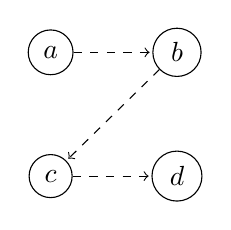
\begin{tikzpicture}
    [every node/.style={draw, circle}]
    \node (a) [] {$a$};
    \node (b) [right = of a] {$b$};
    \node (c) [below = of a] {$c$};
    \node (d) [right = of c] {$d$};

    \draw[dashed, ->, shorten >= 1pt] (a) -- (b);
    \draw[dashed, ->, shorten >= 1pt] (b) -- (c);
    \draw[dashed, ->, shorten >= 1pt] (c) -- (d);

  \end{tikzpicture}
  \caption{An example gossip graph}
  \label{fig:egGossip}
\end{figure}

Let us take this gossip graph to be our example. We want to get to a state where
the formula $K_a (Sbc)$ is true; that is, we want to get to a state where agent
$a$ knows that agent $b$ knows the secret of agent $c$. One call sequence that
will guarantee this is $bc; ab$; $b$ calls $c$ to discover $c$'s secret, and
then $a$ calls $b$. At this point $a$ realises that $b$ knows the secret of $c$,
and hence the formula $K_a (Sbc)$ is satisfied.

This is of course a very high-level description, and is (unfortunately) not hwo
the program will reason about it. Let us step through one application of the
event model \tmc{E} on this graph. In this case, our event model \tmc{E} is the
set of all possible calls; however only three are permitted. This is displayed
in Figure \ref{fig:egGossipE1}

\begin{figure}[h]
  \centering
  \begin{tikzpicture}
    \node(0) [draw, circle] {
        \begin{tikzpicture}
          [every node/.style={draw, circle}]
          \node (a) [] {$a$};
          \node (b) [right = of a] {$b$};
          \node (c) [below = of a] {$c$};
          \node (d) [right = of c] {$d$};

          \draw[dashed, ->, shorten >= 1pt] (a) -- (b);
          \draw[dashed, ->, shorten >= 1pt] (b) -- (c);
          \draw[dashed, ->, shorten >= 1pt] (c) -- (d);

        \end{tikzpicture}
      };


      \node(bc) [draw, circle, below = of 0] {
        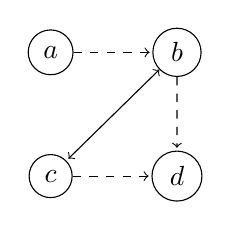
\begin{tikzpicture}
          [every node/.style={draw, circle}]
          \node (a) [] {$a$};
          \node (b) [right = of a] {$b$};
          \node (c) [below = of a] {$c$};
          \node (d) [right = of c] {$d$};

          \draw[dashed, ->, shorten >= 1pt] (a) -- (b);
          \draw[dashed, ->, shorten >= 1pt] (b) -- (d);
          \draw[<->, shorten >= 1pt] (b) -- (c);
          \draw[dashed, ->, shorten >= 1pt] (c) -- (d);
        \end{tikzpicture}
      };

      \node(ab) [draw, circle, left = of bc] {
        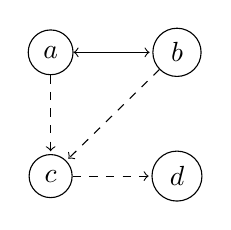
\begin{tikzpicture}
          [every node/.style={draw, circle}]
          \node (a) [] {$a$};
          \node (b) [right = of a] {$b$};
          \node (c) [below = of a] {$c$};
          \node (d) [right = of c] {$d$};

          \draw[<->, shorten >= 1pt] (a) -- (b);
          \draw[dashed, ->, shorten >= 1pt] (a) -- (c);
          \draw[dashed, ->, shorten >= 1pt] (b) -- (c);
          \draw[dashed, ->, shorten >= 1pt] (c) -- (d);

        \end{tikzpicture}
      };
      
      \node(cd) [draw, circle, right = of bc] {
        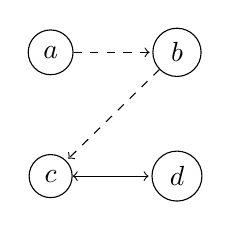
\begin{tikzpicture}
          [every node/.style={draw, circle}]
          \node (a) [] {$a$};
          \node (b) [right = of a] {$b$};
          \node (c) [below = of a] {$c$};
          \node (d) [right = of c] {$d$};

          \draw[dashed, ->, shorten >= 1pt] (a) -- (b);
          \draw[dashed, ->, shorten >= 1pt] (b) -- (c);
          \draw[<->, shorten >= 1pt] (c) -- (d);
        \end{tikzpicture}
      };

      \draw[dashed, ->, shorten >= 2pt] (0) -- (ab) node [midway, left = 2pt] {$ab$};
      \draw[dashed, ->, shorten >= 2pt] (0) -- (bc) node [midway, left = 2pt] {$bc$};
      \draw[dashed, ->, shorten >= 2pt] (0) -- (cd) node [midway, left = 2pt] {$cd$};
      \draw[-, red] (bc) -- (cd) node [midway, below = 2pt] {$~_a$};
    \end{tikzpicture}
    \caption{The gossip graph in \ref{fig:egGossip}, updated with \tmc{E} once.}
    \label{fig:egGossipE1}
\end{figure}

The above diagram shows the three possible states that we could be in afer
making one call from the initial state displayed in \ref{fig:egGossip}. The red
line indicates that agent $a$ cannot distinguish between these two states, as
they were both reached by the execution of a call that agent $a$ was not a
member of. Note that in the algorithm this connection does not exist; it's here
simply for labelling. We can see the three states on the lower row as a Kripke
model, where the three are worlds labelled by their valuation, and the two
connected by the red line are indistinguishable to $a$.

Now say that we wanted to evaluate the formula $\neg S_{ba}$ on the bottom-left
world in Figure \ref{fig:egGossipE1}. This is very straightforward; we just need
to check if $b$ does indeed know $a$'s secret; here it doesn't, and so the world
satisfies $\neg S_{ba}$. But what if we want to evaluate the formula $K_a \neg
S_{ba}$? We need to visit each of the states indistinguishable from our state
and see if $\neg S_{ba}$ holds there. This is currently impossible; we have no
idea whether agent $a$ cannot distinguish between this world and any others, and
certainly no way of reaching those worlds if they are. This is where the
powerset construction comes into play; we pull the indistinguishable states into
the states themselves. Hence, Figure \ref{fig:egGossipE1} becomes Figure
\ref{fig:egGossipE1pset}.

\bigskip

\begin{figure}[h]
  \centering
  \begin{tikzpicture}
    \node(0) [draw, rounded rectangle] {
        \begin{tikzpicture}
          [every node/.style={draw, circle}]
          \node (a) [] {$a$};
          \node (b) [right = of a] {$b$};
          \node (c) [below = of a] {$c$};
          \node (d) [right = of c] {$d$};

          \draw[dashed, ->, shorten >= 1pt] (a) -- (b);
          \draw[dashed, ->, shorten >= 1pt] (b) -- (c);
          \draw[dashed, ->, shorten >= 1pt] (c) -- (d);

        \end{tikzpicture}
      };


      \node(btwn) [below = of 0] {};

      \node(bc) [draw, rounded rectangle, below = of btwn] {
        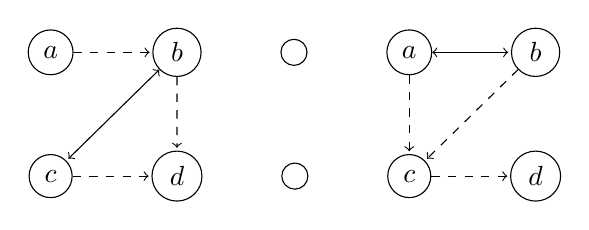
\begin{tikzpicture}
          [every node/.style={draw, circle}]
          \node (a) [] {$a$};
          \node (b) [right = of a] {$b$};
          \node (c) [below = of a] {$c$};
          \node (d) [right = of c] {$d$};

          \node (ln1) [right = of b] {};
          \node (ln2) [right = of d] {};

          \node (aa) [right = of ln1] {$a$};
          \node (ab) [right = of aa] {$b$};
          \node (ac) [below = of aa] {$c$};
          \node (ad) [right = of ac] {$d$};



          \draw[dashed, ->, shorten >= 1pt] (a) -- (b);
          \draw[dashed, ->, shorten >= 1pt] (b) -- (d);
          \draw[<->, shorten >= 1pt] (b) -- (c);
          \draw[dashed, ->, shorten >= 1pt] (c) -- (d);

          
          \draw[<->, shorten >= 1pt] (aa) -- (ab);
          \draw[dashed, ->, shorten >= 1pt] (aa) -- (ac);
          \draw[dashed, ->, shorten >= 1pt] (ab) -- (ac);
          \draw[dashed, ->, shorten >= 1pt] (ac) -- (ad);

        \end{tikzpicture}
      };

      \node(ab) [draw, rounded rectangle, left = of btwn] {
        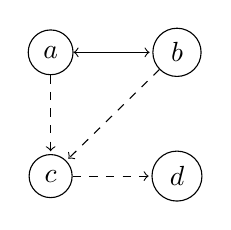
\begin{tikzpicture}
          [every node/.style={draw, circle}]
          \node (a) [] {$a$};
          \node (b) [right = of a] {$b$};
          \node (c) [below = of a] {$c$};
          \node (d) [right = of c] {$d$};

          \draw[<->, shorten >= 1pt] (a) -- (b);
          \draw[dashed, ->, shorten >= 1pt] (a) -- (c);
          \draw[dashed, ->, shorten >= 1pt] (b) -- (c);
          \draw[dashed, ->, shorten >= 1pt] (c) -- (d);

        \end{tikzpicture}
      };
      
      \node(cd) [draw, rounded rectangle, right = of btwn] {
        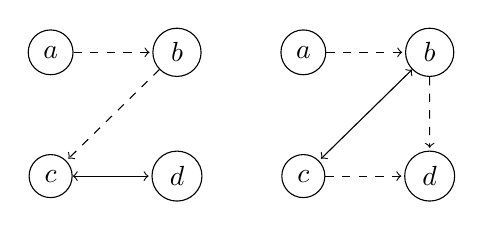
\begin{tikzpicture}
          [every node/.style={draw, circle}]
          \node (a) [] {$a$};
          \node (b) [right = of a] {$b$};
          \node (c) [below = of a] {$c$};
          \node (d) [right = of c] {$d$};

          \node (aa) [right = of b] {$a$};
          \node (ab) [right = of aa] {$b$};
          \node (ac) [below = of aa] {$c$};
          \node (ad) [right = of ac] {$d$};


          \draw[dashed, ->, shorten >= 1pt] (a) -- (b);
          \draw[dashed, ->, shorten >= 1pt] (b) -- (c);
          \draw[<->, shorten >= 1pt] (c) -- (d);

          \draw[dashed, ->, shorten >= 1pt] (aa) -- (ab);
          \draw[dashed, ->, shorten >= 1pt] (ab) -- (ad);
          \draw[<->, shorten >= 1pt] (ab) -- (ac);
          \draw[dashed, ->, shorten >= 1pt] (ac) -- (ad);

        \end{tikzpicture}
      };

      \draw[dashed, ->, shorten >= 2pt] (0) -- (ab) node [midway, left = 2pt] {$ab$};
      \draw[dashed, ->, shorten >= 2pt] (0) -- (bc) node [midway, left = 2pt] {$bc$};
      \draw[dashed, ->, shorten >= 2pt] (0) -- (cd) node [midway, left = 2pt] {$cd$};
      \draw[-, red] (bc) -- (cd) node [midway, below = 2pt] {$~_a$};
    \end{tikzpicture}
    \caption{The automata in Figure \ref{fig:egGossipE1}, now with the
      indistinguishable states in the states.}
    \label{fig:egGossipE1pset}
\end{figure}

The difference between Figures \ref{fig:egGossipE1} and \ref{fig:egGossipE1pset}
now is that the former has all of the states indistinguishable to itself inside
the state. This means that we can evaluate the formula $K_a \neg S_{ba}$ at a
state by simply inspecting the states indistinguishable from the one we're
looking at to check a formula of such form. This is now an extremely
straightforward task! 

An interesting result that arose during implementation and testing of this
algorithm was that the ``actual'' state - that is, the $v$ of the $(v, S)$ pairs
that make up states in the powerset automata - have absolutely no bearing on the
progression of the system. I had originally expected that the actual state would
be treated as a higher-class item than those it was indistinguishable from,
however this was not the case. I suppose this lives up to the nature of the
indistinguishability relation; these states are truly all equal. 

\subsection{Combining Automata}

When we encounter a formula of the form $\phi \land \psi$, where $\phi, \psi \in
\mc{L}_P(\Lambda)$, we may simply construct an automata to solve this formula.
However this is less straightforward when we encounter a formula of the formula
$K_a \phi \land K_b \psi$ \footnote{This occurs very frequently; in this gossip
  problem, we often want to reach a state where every agent knows that everyone
  is an expert.}; in this case, we want to produce powerset automata for $K_a
\phi$ and $K_b \phi$ and then join them back up somehow.

Luckily, intersection for finite automata is well-defined. We give the
definition here. For two automata $A = (\Sigma, Q_A, \delta_A, q_{0A}, F_A)$, $B
= (\Sigma, Q_B, \delta_B, q_{0B}, F_B)$, we define their intersection $A \cap B =
(\Sigma, Q, \delta, q_0, F)$ where $Q = Q_A \times Q_B$, $F = F_A \times F_B$,
$q_0 = (q_{0A}, q_{0B})$ and $\delta(q_A, q_B) = (\delta_A(q_A), \delta_B(q_B))$.

This definition expands in the simple way when we want to take the conjunction
of $n$ automata. 

\bigskip

We have a similar story for negation; given a formula $\neg K_a \phi$, to create
an automata to solve this we build the automata to solve $K_a \phi$ and then
take the complement of this. This consists of simply changing the set of
accepting states. Given automata $A = (\Sigma, Q, \delta, q_0, F)$, we define
$A_\neg = (\Sigma, Q, \delta, q_0, F_\neg)$ where $F_\neg = Q \setminus F$.

\bigskip

To complete our little family of set operations, we should define disjunction
too. Taking the union of automata is, algorithmically, less straightforward than
the intersection; hence we just exploit de Morgan's law and use the identity $A
\cup B = (A^C \cap B^C)^C$. We recognise that when we come to implementation
this may be more costly than some alternative implementation, but for now this
is of little importance. 

\subsection{Searching}

Then given our solving automata, we want to traverse it to find paths that takes
us from the initial state to some successful state. Recall the structure of the
graph \mestar from \secref{subsec:mestar};

\begin{center}
  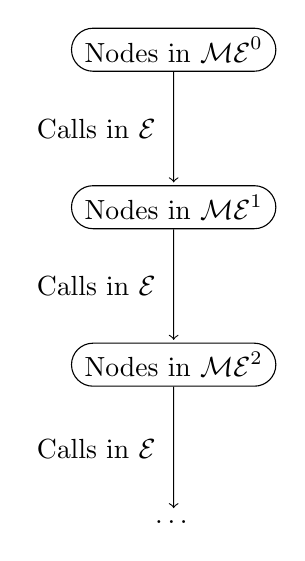
\begin{tikzpicture}[every node part/.style={align=center}]
    \node(0) [draw, rounded rectangle] at (0, 4) {Nodes in $\mc{ME}^0$};
    \node(1) [draw, rounded rectangle] at (0, 2) {Nodes in $\mc{ME}^1$};
    \node(2) [draw, rounded rectangle] at (0, 0) {Nodes in $\mc{ME}^2$};
    \node(3) at (0, -2) {\ldots};

    \draw[->, shorten >= 1pt] (0) -- (1) node [midway, left = 3pt] {Calls in \tmc{E}};
    \draw[->, shorten >= 1pt] (1) -- (2) node [midway, left = 3pt] {Calls in \tmc{E}};
    \draw[->, shorten >= 1pt] (2) -- (3) node [midway, left = 3pt] {Calls in \tmc{E}};
  \end{tikzpicture}
\end{center}

After any kind of powerset, intersection or complement operation, it will still
follow the same shape; we have layers, and as they get deeper more events get
applied to them. One big benefit of this topology is that the resultant graph is
\textit{acyclic}; there is no way we can return to an earlier state.

This is one of the reasons that a breadth-first traversal of the resultant graph
is most suitable for this context. 

\newpage 

\section{Implementation}

We now come to covering the implementation of the algorithm developed in the
previous chapter. We will first give an overview of the structure of the
software and then a summary of all design decisions taken throughout. 

\bigskip

For the implementation of our algorithm, we chose to use Haskell. Haskell is a
lazy functional programming language, which gives us several benefits for this
particular task that other languages lack. 

The first one is the syntax; its functional style lends itself very well to
mathematical definitions. Its list comprehension and pattern matching let us
write code that very closely mimics the original notation, thus erasing a lot of
the difficulty of converting a mathematical definition to code once we have
implemented it. 

Another benefit is its laziness. In our implementation we often use automata
with a ridiculously large state space; however (thankfully) Haskell's laziness
means that we never have to enumerate these states. We only need to access them
when we need them. This saves a lot of processing time, as well as greatly
reduces the space the program takes up.

Its strong type system and typeclasses support us and give us safety guarantees,
preventing us from writing erroneous code that in another language may only be
detected at runtime. A simple example is that in our implementation we cannot
represent a formula that is not well-formed; a more sophisticated one is the
ability to make sure that an epistemic model and an event model span the same
set of atomic propositions and events. Typeclasses help us make code that is
very reusable but also safe; if we wanted to use a new language of atomic
propositions for an existing model, we would only need to give an instance of
the \texttt{Prop} typeclass for our new language and hey presto.

The classification of functions as first-class objects also comes in very
helpful. In the implementation we make the transition function of an FSM a
function $\delta : Q \times \Sigma \rightarrow Q$. Often we want to ``lift'' the
states $Q$ to some other data type, e.g. $P (Q)$. We can very easily unwrap the
datatype $P$ to access the underlying $Q$ and then use the previous $\delta$
function; this would be much more tricky in a language other than Haskell,
however in Haskell it is a very pleasant thing to do.

\bigskip

Haskell offers a simple way to divide each file into a module and import (or
not) a module into another. We give a brief overview of each module in the
system, and highlight notable uses of any of the above language features in this
process. We also highlight any notable design choices made. 

\subsection{\texttt{Model.hs}}

This section is arguably the foundation of the system. Here we implement the
structures defined in \secref{subsec:DEL}; we have the language of our formulae,
Kripke models, Event models and updates thereof.  

In Figure \ref{fig:HaskellModels}, we can see the implementation of both Kripke
models and event models in Haskell. \texttt{states} and \texttt{events}
respectively represent the states and events of the Kripke and Event models, and
\texttt{eprel} and \texttt{evrel} respectively represent the
indistinguishability relations between them. Note that for ease of
implementation we use \textit{partitions} (\cite{EREL}) of sets rather than sets
of pairs. This is done because we regularly want to just access the set of
states we cannot distinguish an item between, and the use of partitions makes
this a much simpler task. 

\begin{figure}[h]
  \centering
  \begin{subfigure}[b]{0.5\textwidth}
    \begin{minted}{haskell}
      data EpistM st prp = Mo {
        states :: [st],                  
        agents :: [Agent],              
        val :: [(st, [Form prp])],         
        eprel :: [(Agent, [[st]])],
        actual :: [st],              
        allProps :: [prp] 
      }
    \end{minted}
    \caption{The Kripke model datatype}
  \end{subfigure}%
~
  \begin{subfigure}[b]{0.5\textwidth}
    \begin{minted}{haskell}
      data EventModel ev prp = EvMo {
        events :: [ev],
        evrel :: [(Agent, [[st]])],
        pre :: ev -> Form prp,
        post :: (ev, prp) -> Form prp
      }
    \end{minted}
    \caption{The Event model datatype}
  \end{subfigure}
  \caption{}
  \label{fig:HaskellModels}
\end{figure}

The user then defines their own \tpre and \tpost-condition functions. One
deviation from the mathematical notation is the addition of the set of agents;
this is purely a pragmatic thing, as it makes certain operations more
straightforward later on.

\begin{figure}[h]
  % \centering
  \begin{subfigure}[b]{0.5\textwidth}
  \begin{minted}{haskell}
    update :: (Eq ev, Prop p) => EpistM (State ev) p -> EventModel ev p -> EpistM (State ev) p
    update epm evm = Mo states' (agents epm) val' rels' (actual epm) (allProps epm)
      where
        states' = [stateUpdate s ev | s <- states epm, ev <- events evm, satisfies (epm, s) (pre evm ev)]
        rels' = [(ag, newRel ag) | ag <- agents epm]
        newRel agent = filterRel states' [liftA2 stateUpdate ss es |
                                          ss <- fromMaybe [] (lookup agent $ eprel epm),
                                          es <- fromMaybe [] (lookup agent $ evrel evm)]
        val' = [(s, ps s) | s <- states']
        ps s = [P p | p <- props, satisfies (epm, trimLast s) (post evm (lastEv s, p))]
        props = allProps epm
  \end{minted}
\end{subfigure}
\caption{The $\mc{M} \times \mc{E}$ function}
\label{fig:update}
\end{figure}

Now we see the definition for the update of a Kripke model with an event model.
Whilst the agents, set of propositions and actual world remain the same, we
update the states, epistemic relations and valuation function in a way very
similar to the definition in \secref{subsec:EventModels}. This is a display of
the merits of Haskell; our implementation stays very close to the specification,
allowing for simple visual verification that the code that we've written matches
the specification. 

\subsection{\texttt{ME.hs}}
\label{sec:MEHaskell}

We now come onto the module that handles construction of the automata \mestar.
This is a slightly more interesting case.

In this module we make use of one of the many language extensions Haskell offers
us, namely \texttt{MultiParamTypeClasses}.

\begin{figure}
  \begin{minted}{haskell}
    class (Ord st, Prop p) => EvalState st p where
    evalState :: Form p -> st -> Bool
  \end{minted}
\end{figure}

This lets us ensure in our functions that the propositions we're using can be
evaluated at the states we want them to be evaluated at. This prevents us from
trying to evaluate formula of a certain language on a world it is incompatible
with.

\subsection{\texttt{FSM.hs} and \texttt{FST.hs}}

These two modules hold our finite state machines. Given how much of the
algorithm relies on state machines, it was very important in development to have
a reliable structure for state machines. Furthermore, we needed to do some
non-standard operations on the machines we implemented (namely, the composition
mentioned in \secref{subsubsec:TransducerComposition}). To do this easily we need
low-level access to the states and a good understanding of the library. 

The two libraries that seemed most suitable were \cite{HaskellFST} and
\cite{HaskellMachines}. However, in both libraries, there seemed to be far too
much to take in; it felt like the time spent trying to understand how to use the
library (particularly in the latter) would far outweigh any potential benefit
gained from using them. Furthermore it was particularly unclear how we would go
about implementing our single-state composition as mentioned above.

\bigskip

Fortunately, implementation of these finite-state machines is incredibly
straightforward. We can see in \figref{fig:FSMFST} that the datatypes nearly
identically mimic the tuple definitions in \secref{subsec:Transducers}.


\begin{figure}[h]
  \centering
  \begin{subfigure}[b]{0.5\textwidth}
    \begin{minted}{haskell}
      data FSM ch st = FSM {
        alphabet :: [ch],              
        states :: [st],               
        transition :: (st, ch) -> Maybe st,
        initial :: [st],            
        accepting :: st -> Bool    
       }
    \end{minted}
    \caption{The FSM datatype}
  \end{subfigure}%
~
  \begin{subfigure}[b]{0.5\textwidth}
    \begin{minted}{haskell}
      data FST ch st = FST {
        alphabet :: [ch],                     
        states :: [st],                       
        bitransition :: (st, ch) -> [(ch, st)],
        initial :: [st],                      
        accepting :: st -> Bool              
      }
    \end{minted}
    \caption{The FST datatype}
  \end{subfigure}
  \caption{}
  \label{fig:FSMFST}
\end{figure}

Our FSM's transition returns a \texttt{Maybe st} to encode that it is
\textit{nondeterministic}; meaning that it is not guaranteed to return a state
on a transition. This comes in useful in practise when we have as input to
$\delta$ some pair $(w, e)$ where $e$ is not permitted at $w$. In this case,
$\delta(w, e) = \texttt{Nothing}$. An example of this is a call $ij$ in the
gossip problem where $i$ does not know $j$'s phone number.

Similarly, the FST transition returns a list of $(e, q)$ pairs. This again
encapsulates the nondeterminism of the FST. This is useful in the case of
\secref{subsubsec:TransducerComposition}, where we want to return from
$\Delta(q, e)$ the set of all pairs $(e', q')$ where $e'$ is some event
indistinguishable from $e$ and $q'$ is the state reached by making the
transition $\delta(q, e')$. 

\subsection{\texttt{Powerset.hs}}

\begin{wrapfigure}{r}{0.5\textwidth}
  \begin{center}
    \begin{minted}{haskell}
      data PState st = PList [PState st] 
                     | PCon (PState st) 
                            [PState st] 
                     | PVar st 
    \end{minted}
  \end{center}
  \caption{The \texttt{PState} datatype.}
\end{wrapfigure}

This module contains all of the functions pertaining to the powerset
construction, as specified in \secref{sec:PowersetAdapted}.

As before, we keep definitions very close to the mathematical specification. We
introduce a new datatype, \texttt{PState}, which holds our states in the
powerset. \texttt{PVar} is the ``atomic'' constructor, and it is here that the
formulae are actually evaluated. \texttt{PCon} represents an actual state and
the set of states indistinguishable from this state; such states arise when we
want to evaluate a modal formula. Finally the \texttt{PList} constructor is used for
conjunctions; we pass through all of the states in the list simultaneously.

The reason we do this is so that we can create our automata recursively.
Consider the function in \figref{fig:createSolvingAutomata}\footnote{For clarity
  and brevity, we omit some of the supporting function calls, and also omit some
  of the cases.}. This is the function we use to create the automata we traverse
to find successful sequences of events; it pattern matches on the formula given
in the first argument to decide the ``shape'' of the returned automata.

Let us first consider the bottom case. We receive some formula, e.g. $S_{ab}
\land S_{bc}$. Then we build an automata \mestar whose successful states are
those which satisfy the formula $S_{ab} \land S_{bc}$, through the procedure in
\secref{sec:MEHaskell}. 

If it receives a formula $K_a \phi$, then we call the \texttt{buildPSA}
function, which performs the powerset creation process as detailed earlier. Note
that it does so with the automata that solves the formula $\phi$, invariant of
the form of $\phi$ - it could be an atomic proposition or another modality, or a
conjunction of modalities. 

\begin{figure}[h]
  \centering
    \begin{minted}{haskell}
      cSA :: Form p -> EpistM (State ev) p -> EventModel ev p
             -> FSM (Character ev) (PState (QState p))
      cSA form@(K agent phi) ep ev
        = buildPSA 
                   (cSA phi ep ev) 
                   (buildComposedSS agent ep ev (cSA phi ep ev)) 

      cSA (Not phi) ep ev = complement $ cSA phi ep ev tfilter

      cSA (And phis) ep ev = case includesK (And phis) of
        True  -> toPList $ intersection $ map (\phi -> cSA phi ep ev) phis
        False -> makeP $ buildMEStar (And phis) ep ev

      cSA phi ep ev = makeP $ buildMEStar phi ep ev
    \end{minted}
  \caption{The \texttt{createSolvingAutomata} function.}
  \label{fig:createSolvingAutomata}
\end{figure}

\newpage

\section{Evaluation}

\subsection{Plan for Testing}

Throughout development we used the Haskell library \texttt{HUnit}. This provides
a wealth of combinators that we can use to tersely write unit tests for our
functions. This was used in a standard manner; before implementing a function we
would write tests for it, and then implement the function, ensuring it passes
all tests and as such functions correctly.

\bigskip

However, more interesting is our plan for functional testing. This is the part
of testing in which we check that the system \textit{correctly functions}, and
will tell us if what we have implemented is correct or not.

Although our system is capable of planning for any epistemic model and
propositional event model, we chose to test solely on gossip models. This is
for several reasons:

\begin{itemize}
\item Gossip models cover every part of the system (epistemic models, \mestar,
  the powerset construction) and as such give us maximal test coverage;
\item Testing with a certain class of models tells us that all of the code
  works; the algorithm does not depend on what the particular model is. Hence if
  we know it is correct for a certian class of models, it will also be correct
  for any other class of models;
\item We have an existing model checker speciailised for the Gossip problem that we can use
  (\cite{GithubGossip});
\item It is the class of models best understood by myself; hence if an error
  arises it should be quite easy to understand. 
\end{itemize}

This in mind, we chose to use \cite{GithubGossip} to verify our results. It was
chosen over the other two tools (\cite{SMCDEL}, \cite{DEMO-S5}) due to its ease
of accessibility; we can provide it with just a list of lists encoding who knows
who's phone number, and it will produce an epistemic model for us. This is very
easily produced from the epistemic models in our software. This is a sharp
contrast to \cite{SMCDEL}, which uses a text file based input - output interface
which would have added significant complication to the testing process. We could
have very easily used \cite{DEMO-S5}, given the similarity betweeen the Kripke
models in our code and in \cite{DEMO-S5}, however \cite{GithubGossip} was
eventually chosen due to the conversion between the two representations of a
Gossip graph being so straightforward. The last thing we wanted to do was create
some kind of bug within the testing software!

\subsection{Testing Frameworks}
\label{sec:TestingFrameworks}

The next decision to be made was how to actually go through with the testing
process. Haskell offers the seminal property-based library \texttt{QuickCheck},
which, when given a function $\texttt{a} \rightarrow \texttt{Bool}$ and a way to
generate arbitrary values of type \texttt{a}, will test the function on these
arbitrary values and ensure that the function returns $True$. All that we need
to provide in order to generate these arbitrary values is an instance of the
\texttt{Arbitrary} typeclass. We can see an example of this in \figref{fig:Arbitrary}.

\begin{figure}[h]
  \centering
  \begin{minted}{haskell}
      instance Arbitrary (EpistM StateC GosProp) where
        arbitrary = standardEpistModel agents <$> (sublistOf $ allNumbers agents)
  \end{minted}
  \caption{An \texttt{Arbitrary} instance for an epistemic model.}
  \label{fig:Arbitrary}
\end{figure}

Once we have this, we perform a breadth-first search on the automata generated
by this epistemic model and the target formula in order to find either a path
that takes us to a successful state, or a response telling us that no such path
exists. Whatever the outcome, we then send this result and the original model to
a function that converts our model to a model in the style of
\cite{GithubGossip} and uses the model checker there to verify our answer.

\bigskip

\texttt{QuickCheck} was working well, however I quickly wanted to be able to
check for every possible gossip graph. QuickCheck will sometimes repeat
instances \footnote{To verify this, simply open up your nearest Haskell REPL,
  import \texttt{QuickCheck}, and run the line of code \texttt{verboseCheck
    (($\lambda$ s -> s == s) :: Bool -> Bool)}}; hence to get every single
possible gossip graph I simply created a list with every single graph in and
performed the same process of using the model checker from \cite{GithubGossip}
on each graph.

\bigskip

The creation of gossip graphs is very straightforward; we just produce some set
of propositions $N = \left\{ N_{ij} \right\}$ where $\forall N_{ij} \in N, i
\not = j$. We only look for cases where the agents start out not knowing the
phone number of any agent apart from each other - we call these
\textit{phonebook} graphs. There are a few reasons for this;

\begin{itemize}
\item These cases are the only interesting ones. Any gossip graph where some
  agent already knows the secret of another will either have the same call
  sequence or a shorter one than the same graph, where no agent knows the secret
  of any other.
\item These cases are the most faithful to the applications of the gossip
  problem in reality.
\item On a pragmatic note, it is more straightforward to convert phonebook
  graphs to the representation in \cite{GithubGossip} than non-phonebook graphs.
\end{itemize}

\subsection{Profiling}

One of the project aims was to perform a space and time analysis of our
implemented system. We have a number of reasons to do this;

\begin{itemize}
\item Firstly, it lets us give a quantitative comparison of our program's
  efficacy compared to the existing tools.
\item It also lets us find the parts of our code to try and optimise. It is said
  that a program spends $90\%$ of its time in $10\%$ of its code; a profiler helps
  us find this $10\%$.
\item It also lets us find the weaknesses of our program in comparison to other
  tools, and as such find the weaknesses of the algorithm put forward. 
\end{itemize}

In order to do this we used the profiling tool built into GHC. This gives us a
detailed cost-centre breakdown of in which functions the majority of the time is
spent, as well as the space used by these functions. We can see an example in
\figref{fig:costcentre}.

\begin{figure}[h]
% This is after.prof.   
\begin{minted}{text}
	Mon Apr 15 14:23 2019 Time and Allocation Profiling Report  (Final)

	   Main +RTS -p -RTS

	total time  =        1.46 secs   (1457 ticks @ 1000 us, 1 processor)
	total alloc = 1,036,538,824 bytes  (excludes profiling overheads)

  COST CENTRE            MODULE                 %time %alloc

  models                 ME                      20.7    3.3
  compare                Model                   14.3    0.0
  compare                ME                       9.7   22.0
  meTrans                ME                       9.2   11.5
  enqueue                BFSM                     5.2   10.8
\end{minted}
  \caption{An example cost centre output from GHC.}
  \label{fig:costcentre}
\end{figure}

In the following section, we will give an analysis of the time and space used
for several sizes of gossip graph and several different winning formulae, and
compare them against the corresponding results in \cite{GithubGossip}. We use
\cite{GithubGossip} as it is the only tool capable of planning.

Note that the way that our tool and \cite{GithubGossip} plan are quite
different. In our tool we return just one successful sequence of events; in
\cite{GithubGossip} all possible sequences are returned. It is unclear how to
use the latter tool to return just one; hence in the interests of fairness we
just use the function that returns all the possible paths.


\subsubsection{Profiling Framework}

In our profiling we will generate random graphs as in
\secref{sec:TestingFrameworks}, use them in both tools and then take averages.
This is because certain graphs will take much less time than others
\footnote{Consider a graph where no one knows anyone elses phone number; both
  tools will very quickly decide that there is no successful path through this.
  A graph where there is a successful path will take much longer to compute the
  path, in comparison.}, and we want to give the most accurate statistics.

We then perform the planning process on the generated gossip graph. As mentioned
earlier we run for some amount of graphs and then take the average.

\subsubsection{Profiling Results}

When profiling, we generated gossip graphs of size 4 (by which we mean graphs
with 4 agents in). This is not an arbitrary number; 4 is the smallest
``interesting'' gossip graph, meaning the smallest graph where a call occuring,
not including some arbitrary agent $a$, has interesting other options; it could
be from $b$ to $c$, or $b$ to $d$, or $c$ to $d$ \footnote{Compare this to a
  gossip graph of size 3; a call not involving some agent $a$ can only be from
  either $b$ to $c$ or $c$ to $b$.}. Furthermore, graphs of size greater than 4
take an impractically long time - it is in the interests of time to use graphs
of size 4.

When testing, the variable that we varied is the complexity of target formula.
This might seem like an odd choice, but it is well-motivated;

\begin{itemize}
\item In \cite{AutomataTechniques}, it is postulated that the runtime and space
  complexity of the program is $k$-exponential, where $k$ is the maximal depth
  of the nesting of our $K$ modalities. We want to investigate this claim.
\item This will give us a handle to compare the methodologies in the two tools,
  and spot the differences in how knowledge is handled.
\end{itemize}

\bigskip

We tabulate the results here. We abbreviate the statement ``all agents are
experts'' to the propositional variable $E$. 

\begin{table}[h]
  \centering
  \begin{tabular}{|c||c|c|c|}
    \hline
    & $E$ & $ K_a E$ & $K_b K_a E$  \\ \hline 
    Our tool   & 0.00917s, 7.36Mb  & 0.0150s, 10.15Mb & 0.0239s, 14.12Mb \\ \hline 
    Other tool & 0.1449s, 251Mb & 0.724s, 1.25Gb & 3.849s, 6.425Gb \\ 
    \hline
  \end{tabular}
  \caption{Profiling Results between our tool and \cite{GithubGossip}}
  \label{tab:Proflining1}
\end{table}

We can clearly see that our tool is much more time and space efficient than the
existing tool. However this is a quite straightforward victory; the other tool
enumerates \textit{all} of the possible paths through a gossip graph (for a
graph of size 4, there thousands of these), and then checks the success of each
one. Compare this to our tool, which simply find the first, shortest, successful
path it can take to reach some successful state.

Hence to get a more accurate comparison, we slightly modify the code of the
existing tool to exit once it finds a single successful path. This means that it
closer mimics our tool, and as such will let us get a better performance
comparison between the two. 


\begin{table}[h]
  \centering
  \begin{tabular}{|c||c|c|c|c|}
    \hline
    & $E$ & $ K_a E$ & $K_b K_a E$ & $K_c K_b K_a E$ \\ \hline 
    Our tool   & 0.00917s, 7.36Mb  & 0.0150s, 10.15Mb & 0.0239s, 14.12Mb & 0.0965s, 65.094Mb \\ \hline 
    Other tool & 0.0006s, 0.694Mb  & 0.0015s, 2.006Mb & 0.0042s, 4.6104Mb & 0.0074s, 11.077Mb \\
    \hline
  \end{tabular}
  \caption{Profiling Results between our tool and \cite{GithubGossip}, with modification}
  \label{tab:Proflining2}
\end{table}

We see that the other tool now outperforms ours, in both space and time
efficiency. 

\subsubsection{Conclusions from Profiling}

\begin{wrapfigure}{r}{0.5\textwidth}
  \begin{center}
    \begin{minted}{haskell}
      models :: Prop p => Set.Set p -> Form p -> Bool
      models _  Top         = True
      models ps (Not form)  = not $ models ps form
      models ps (P form)    = Set.member form ps
      models ps (Or forms)  = any (models ps) forms
      models ps (And forms) = all (models ps) forms
    \end{minted}
  \end{center}
  \caption{The \texttt{models} function}
  \label{fig:modelsfunction}
\end{wrapfigure}



Through looking at the cost centres given to us by GHC, we can see where our
program spends the bulk of the time computing. In our tool, the culprit is
\texttt{models}, which can be seen in \figref{fig:modelsfunction}. Unfortunately
there's no more we can do to speed up this function \footnote{Short of using a
  HashSet, which gives us quicker lookup times.}, suggesting that the problem
lies in the amount of times we call it. The function is one of the essential
parts of the program; it lets us move from state to state.

The issue seems to arise from the final part of the definition of transitions in
\mestar. Recall that this is defined as:

\begin{equation} \label{eq:delta1}
  \delta(q_v, e) = q_{v'}, \text{where } v' = \{p \in \Lambda \mid v \models \post(e, p)\}
  \text{ if } 
  \models \pre(e)
\end{equation}

\noindent where, given a world where a set of propositions $v$ is true and an
event $e$, we go through each proposition $p$ in the set of propositions for the
current model and check if the set of propositions $v$ \textit{model} the postcondition
of the given proposition $p$ and the event $e$. This occurs every time we wish
to make a transition between two sets in our automata; clearly, this piece of
code is being called a lot. However, this does not seem to be a particularly bad
thing in itself; rather the opposite, it seems essential that this piece of code
would be called a lot.

\bigskip

To understand the differences, we mainly need to consider the algorithmic
differences. The other tool first enumerates the possible set of call sequences
in a depth-first manner, after which it finds the first successful sequence of
these calls. It does this latter task like a conventional model checker, and as
such can use more powerful model checking techniques. In contrast, our tool
performs a slightly different task; it builds a structure with which it can find
paths through the gossip graph, and then finds the shortest.

The point at which this difference is really shown is in the generation of
indistinguishable states. In our tool we progressively keep track of the states
indistinguishable from our current one, and update each of these states with
each transition, leading to a lot of time spent in the \texttt{models} function.
In contrast, the other tool takes the string of calls to be checked against and
generates all of the other strings of calls indistinguishable to it, and then
checks if these model the target formula. The latter technique is much more
computationally efficient than ours; the generation of these indistinguishable
call sequences is much more straightforward and requires much less heavy lifting
than maintaining this set of indistinguishable states.

% However, the method of computing these other call sequences is one that can only
% be effectively utilised when we know the 

One might ask why we don't copy this method of simply maintaining the set of
strings of indistinguishable events which could have happened in the states of
our automaton. This is a fine idea, however a problem arises when we come to
considering the successful states. In the other tool it is known that the
sequence of calls is ``final'', in the sense of a model checker - we want to
know if this is successful or it isn't. But in ours we only stop either when we
can make no more calls, or we are in a successful state. As such, we need to
know if we are in a successful state \textit{every time we enter one}, and the
only way we can do this is by performing each string of indistinguishable calls
on the initial state and evaluating the target formula at the resultant states;
it is clear that this will be less efficient.

\bigskip

Another method we spend a lot of time on is the BFSM method \texttt{enqueue}. In
this we take the existing queue and append onto it the set of states that are
next to be visited. This function uses a lot of memory and time as it has two
memory-costly functions inside it; namely \texttt{filter} and \texttt{(++)}.
This was an interesting function to investigate and try and optimise. We only
need to perform two actions on our queue:

\begin{enumerate}
\item Read an item from the front
\item Append items onto the back
\end{enumerate}

In Haskell, list concatenation has runtime $O(n)$, where $n$ is the length of
the list being appended to\footnote{I.e., in the command \texttt{xs ++ ys}, $n$
  is the length of \texttt{xs}.}. This is far from ideal - however the
\texttt{Data.Seq} package offers us constant-time access to the first and last
element of a sequence. This seems like it would be perfect for our situation,
however \textbf{for some reason currently beyond me} the time nearly doubles and
the space used balloons.

\bigskip

Another thing we could have used to reduce computation is the monotonicity of
the propositions true at a state. At a state in the gossip protocol, if some set
$v$ of propositions are true and we make some call $e$, then the set of
propositions at the state we move to, $v'$, is guaranteed to be a superset of
$v$. Consider what this means; there is no phone call that can be made that will
make anyone know any \textit{less}. Hence we could change Equation
\ref{eq:delta1} to

\begin{equation} \label{eq:delta2}
  \delta(q_v, e) = q_{v'}, \text{where } v' = \{p \in \Lambda \setminus v \mid v \models \post(e, p)\} \cup v
  \text{ if } 
  \models \pre(e)
\end{equation}

This is because we know that the propositions in $v$ will be true at the state
$\delta(q_v, e)$; hence we do not need to check again whether or not they will
be true. 

However I fear this would be an irresponsible change to make to our code.
Remember that we do not want our system to solely plan for the Gossip problem;
rather we want it to be capable of doing so for \textit{any} epistemic model and
propositional event model. We have an example of a model where this occurs in
\figref{fig:cointoss}; although this is quite a toy example, it does indeed show
that such cases are possible. In the interests of portability then, it would be
unwise to make such a change. 

\subsection{Negatives of Design}

\newpage

\section{Conclusion}

We now take some time to reflect on the work done in this project. Our
overarching aim in the project was to design an implement a system with which we
can perform epistemic planning. This document's ordering reflects the order in
which the challenges of the project were accomplished; we first reviewed the
literature, then designed the algorithm, and then implemented it. Chapters 2, 3
and 4 are respectively dedicated to each subtask.

\bigskip

In Chapter 2, we explained the concepts necessary to understand the algorithm
put forward. When starting work on this project the understanding of the
processes put forward in the literature was the first major difficulty, and as
such care has been taken in the writing process to make these definitions as clear
as possible. 

\bigskip

In Chapter 3, we put forward the algorithm designed to perform the task of
planning.

\subsection{Future Work}

It is clear to see that our system is very slow; when run on a gossip graph with
greater than 6 agents the takes so long that it's not worth waiting for the
results. Whilst there is scope for implementation-based
optimisations\footnote{By which we mean optimisations like changing a
  \texttt{Set} to a \texttt{HashSet} and so on.}, this is mainly due to the
algorithm; in \cite{AutomataTechniques} it is shown that the propositional
epistemic planning problem is in \textsf{$k + 1$-EXPTIME}, where $k$ is the
depth of the deepest-nested knowledge operator. 

The method that we use is very explicit; we will always explore a branch, no
matter what its state is. We may be wasting computation by either exploring a
branch that is never going to succeed, or is identical to another branch. It
would be interesting to see the implementation of some checker for recomputed
branches, a la dynamic programming.

\bigskip

It also seems possible that there's scope for a symbolic approach, like in
\cite{MalvinThesis}.

%%% Bibliography %%%%%%%%%%%%%%%%%%%%%%%%%%%%%%%%%%%%%%%%%%%%%%%%%%%%%%%%%%%%%%%%

\newpage

\printbibliography[title={Bibliography}]



\end{document}
